%!TEX encoding = UTF-8 Unicode
%\part{Design of Excitation System}
\chapter{Design of Excitation System for Simulating Dynamic Loads}
\label{chap:6}
\section{Design Controller of Excitation System for Simulating Wind Responses}


In this section, simulation of wind-induced responses of a building structure using linear mass shaker (LMS) and active tuned mass damper (ATMD) as an actuator is conducted as shown in Figure~\ref{fig:6-1}. For the linear actuator to keep the structure in the target response trajectory, an inverse transfer function of a structural response to the shaker force is obtained using a state space form governing equation of the structure, and the discrete Fourier transform of structural response is performed. Filter and envelope function are used such that the error between wind and actuator induced responses is minimized by preventing the shaker from actuating unexpected modal responses and initial transient responses. The effectiveness of the proposed method is verified through a numerical example of a 76 story-benchmark building excited by wind load of which deterministic time history is given. The effect of the type of the target structural response on a convergence of the actuator force signal and the error magnitude is investigated.

\begin{figure}[ht]
\centering
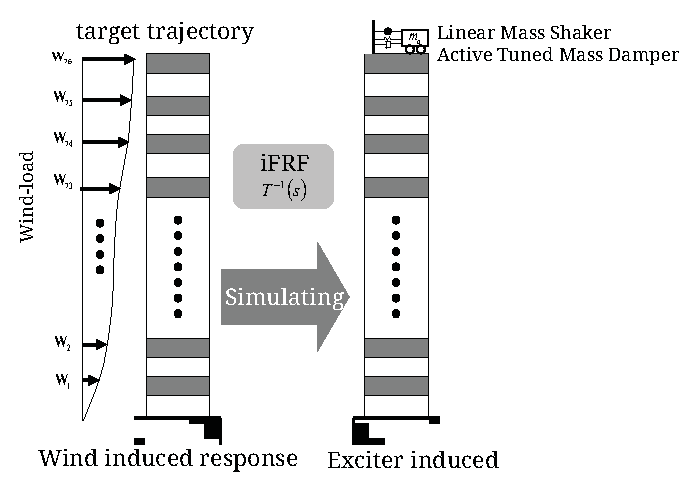
\includegraphics[width=1\textwidth] {figure/6-1.eps}
\caption{Scheme of simulation of wind induced responses using LMS and ATMD}
\label{fig:6-1}
\end{figure}

\subsection{Force of actuator}
The state space form equation of a structure excited by wind load $f$ and the shaker generated force $u$ of size $r$ is as follows.

\begin{equation}
\begin{aligned}
\dot{\matr{z}} &=\matr{A}\matr{z}+\matr{B}_{f}f + \matr{B}_{u}u \\
y &= \matr{C}\matr{z}+\matr{D}_{f}f+\matr{D}_{u}u
\end{aligned}
\label{eq:6-1}
\end{equation}

where, $z$ is the state vector and $y$ is the output vector of size $m$. The output transfer function to $f$ or $u$ is given by

\begin{equation}
\begin{aligned}
\matr{T}_{yf} &= \matr{Y}_{f}(s)\matr{F}(s)^{-1} = \matr{C}\left(s\matr{I}-\matr{A}\right)^{-1}\matr{B}_{f} \\
\matr{T}_{yu} &= \matr{Y}_{u}(s)\matr{U}(s)^{-1} = \matr{C}\left(s\matr{I}-\matr{A}\right)^{-1}\matr{B}_{u} \\
\end{aligned}
\label{eq:6-2}
\end{equation}

where the scalar $s$ is a complex variable $j\omega$ . The inverse of $\matr{T}_{yu}$ exists only if $r$ equals to $m$ and the Laplace transform of $u$ providing the identical output to wind load induced one is determined as

\begin{equation}
\begin{aligned}
\matr{U}(s)&=\matr{T}_{yu}^{-1}\matr{Y}_{u}(s)\\
&=\matr{T}_{yu}^{-1}\matr{T}_{yf}\matr{F}(s)
\end{aligned}
\label{eq:6-3}
\end{equation}

when $r$ is smaller than $m$, the number of structural responses which can be modulated by $u$ is restricted to $r$ and target structural response should be selected. The Laplace transform of input realizing the target response $\bar{y}$ of size $r$ is

\begin{equation}
\begin{aligned}
\hat{\matr{U}}(s)&=\hat{\matr{T}}_{yu}^{-1}\hat{\matr{Y}}_{u}(s)\\
&=\hat{\matr{T}}_{yu}^{-1}\hat{\matr{Y}}_{f}(s)\\
&=\hat{\matr{T}}_{yu}^{-1}\hat{\matr{T}}_{yf}F(s)
\end{aligned}
\label{eq:6-4}
\end{equation}

where, $\hat{\matr{T}}_{yu}^{-1}$ is a sub-matrices of $\matr{T}_{yu}^{-1}$ is constructed by extracting the columns in $\matr{T}_{yu}^{-1}$ corresponding to the target response.

\subsubsection{Filter and evelop function}
The transfer function of structural response may have frequency intervals in which the magnitude is as small as zero, and in those intervals, the magnitude of the inverse transfer function increases infinitely. Because the input force is calculated by the product of the inverse transfer function and the output signal, significant input force may be calculated in order to realize the small magnitude of output components corresponding to the intervals. This force implies that the shaking system becomes very sensitive to the slight frequency variation of the output signal resulting from measurement noise and spectral leakage which is inevitable in signal processing using discrete Fourier transform, and then unnecessarily high input energy excites unexpected frequency response such that target response may not be induced. Particularly, low-frequency component leads to a large stroke of the shaker. In this study, following band-stop filter (BSF) using cosine function is used to prevent the unexpected frequency response from occurring.

\begin{equation}\label{eq:6-5}
\hat{\matr{U}}_{p}(\omega) = G(\omega)\hat{\matr{U}}(s)
\end{equation}

where,
\begin{align}
G(\omega) &= \frac{1-a_{co}}{2}cos \left( \frac{2\pi}{\omega_{2}-\omega_{1}}\omega \right) + \frac{1+a_{co}}{2}\label{eq:6-6}\\
a_{co} &=\left\{\begin{array}{lr} \omega < \omega_{1} &: 1 \\ \omega_{1} \leq \omega \leq \omega_{2} &: 0 \\ \omega > \omega_{2} &: 1\end{array} \right.
\label{eq:6-7}
\end{align}

where, $\omega_{1}$ and $\omega_{2}$ are frequencies defining the cut-off frequency interval, and $a_{co}$ is gain value of the cut-off frequency. Figure~\ref{fig:6-2a} shows the shape of the band-stop filter

In discrete Fourier transform dealing with the finite duration discrete signal as an infinite one multiplied by a rectangular window, the original signal in time domain is distorted especially in initial and final time intervals. This distortion can be reduced by using an envelope function such that the given deterministic wind load has ascending and descending time intervals. Although the envelope function changes the deterministic wind load, the effect of this another distortion would be trivial in evaluating the characteristics of wind load induced response because the grave concern is generally in the intermediate time of the total loading duration when the peak response is expected to occur. Figure~\ref{fig:6-2b} shows the shape of the envelope function used in this study.

\begin{figure}[!ht]
\centering
\subfigure[The shape of the band-stop filter]{
   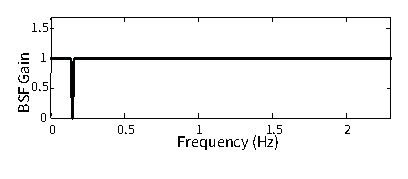
\includegraphics[width=0.45\textwidth] {figure/6-2a.eps}
   \label{fig:6-2a}
 }
 \subfigure[The shape of the envelop function]{
   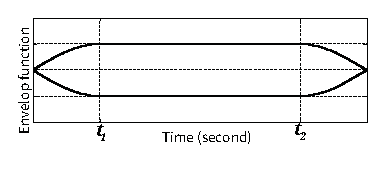
\includegraphics[width=0.45\textwidth] {figure/6-2b.eps}
   \label{fig:6-2b}
 }
\caption{Exciter gain shape of the band-stop filter and the envelop function.}
\label{fig:6-2}
\end{figure}

\subsection{Numerical Example}
\subsubsection{76 story wind-induced benchmark buildings}

The wind-induced response simulating actuator is applied to a 76-story 306 meters office tower benchmark building which is slender with a height to width ratio of $306.1/42= 7.3$. Because the deterministic across-wind load data is given through wind tunnel tests for this benchmark building, the force of the actuator realizes target across-wind induced structural response can be calculated using Eq.~\eqref{eq:6-4}. In order to reduce numerical computation time, a 23 degree of freedom (DOF) state reduced-order system model proposed by \citet{yang2004benchmark}. is used in this study. The wind load vector is modeled physically by lumping wind forces on adjacent floors at the locations that correspond to the 23 DOF model. Figures~\ref{fig:6-3a},~\ref{fig:6-3b} shows the plan view and elevation view of the 76th benchmark building and Figures~\ref{fig:6-3c},~\ref{fig:6-3d} show the mode shape of first three mode of the structure and time history of wind-load.

\begin{figure}[!ht]
\centering
\subfigure[Plan View of the 76-Story Building]{
   \includegraphics[width=0.45\textwidth] {figure/6-3a.eps}
   \label{fig:6-3a}\hfill
 }
 \subfigure[Elevation View of the Building.]{
   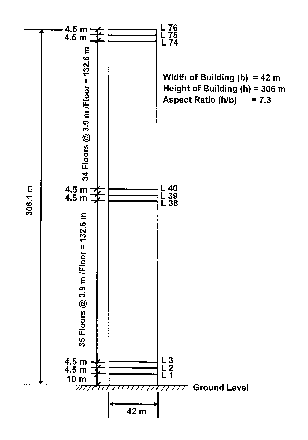
\includegraphics[width=0.45\textwidth] {figure/6-3b.eps}
   \label{fig:6-3b}
 }
\subfigure[Mode shapes of First Three Modes of the Building.]{
   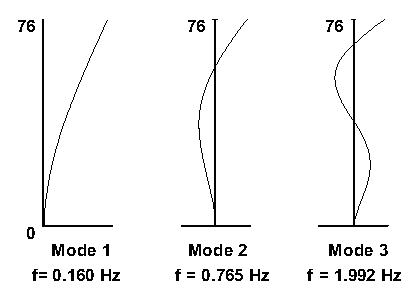
\includegraphics[width=0.45\textwidth] {figure/6-3c.eps}
   \label{fig:6-3c}\hfill
 }
 \subfigure[Time Histories of Wind Load on Floors 50, 60 and 70; $W_{50}$, $W_{60}$ and $W_{70}$.]{
   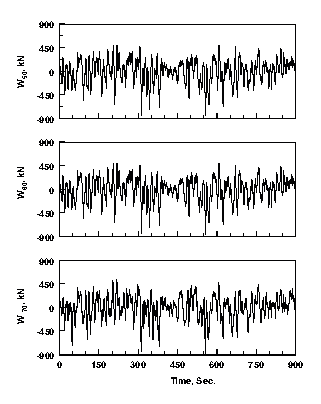
\includegraphics[width=0.45\textwidth] {figure/6-3d.eps}
   \label{fig:6-3d}
 }
\caption{76th story benchmark model.}
\label{fig:6-3}
\end{figure}

\subsection{Error evaluation criteria}
In order to verify the effectiveness of proposed method through the comparison between the wind and actuator induced structural responses, two error criteria are considered in time and frequency domains, respectively.
In time domain, the normalized tracking error is defined as 

\begin{equation}\label{eq:6-8}
e_{t} = \frac{1}{n}\sum_{i=0}^{n-1}\sqrt{\left\{ z_{a} \left(i\Delta t \right) -z_{f}\left(i\Delta t\right) \right\}^{2}}  \Biggm/ \text{max} \left[\sqrt{z_{f}\left(i\Delta t\right)^{2}} \right]
\end{equation}

where, $\Delta t$ denotes time interval, $n$ denotes the data number. $x_{a}\left(i\Delta t\right)$ and $x_{f}\left(i\Delta t\right)$ are, respectively, actuator and wind induced structural response at the $i$th time step.

In frequency domain, the normalized tracking error is defined as

\begin{equation}\label{eq:6-9}
e_{f} = \frac{1}{N}\sum_{i=1}^{N}\sqrt{\left| Z_{a} \left(\omega_{i} \right) -Z_{f}\left(\omega_{i}\right) \right|^{2}} \Biggm/ \text{max} \left[\sqrt{\left|Z_{f}\left(\omega_{i}\right)\right|^{2}} \right]
\end{equation}

where $N$ is the number of frequency response data, and $X_{f}(\omega)$ and $X_{t}(\omega)$ are discrete-Fourier transformation of $\ddot{x}_{f}(t)$ and $\ddot{x}_{t}(t)$, which $E\left[\epsilon_{f}(\omega)\right]$ is normalized mean tracking error in frequency domain.

\subsubsection{LMS excitation}
In this subsection, an LMS which can produce arbitrary desired force is used as an actuator. LMS is assumed to have a mass of 500 metric ton and be installed at 76th floor. The mass is identical to that of an ATMD used as a vibration dissipation device for the benchmark problem. The mass is about 45\% of the top floor mass, which is 0.327\% of the total mass of the building.

Figures~\ref{fig:6-4a} and \ref{fig:6-4b} show the transfer function of the 75th floor acceleration and displacement responses. It is observed that acceleration transfer function in Figure~\ref{fig:6-4a} has zero near the each modal natural frequency with slightly larger value than the corresponding natural frequency. Especially the zero exists near the first modal frequency which is expected to dominate the overall wind-induced structural responses.

\begin{figure}[!ht]
\centering
\subfigure[75th story acceleration transfer function.]{
   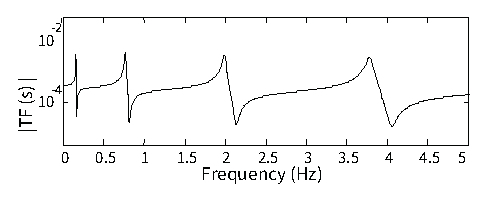
\includegraphics[width=0.8\textwidth] {figure/6-4a.eps}
   \label{fig:6-4a}
 }
 \subfigure[75th story displacement transfer function.]{
   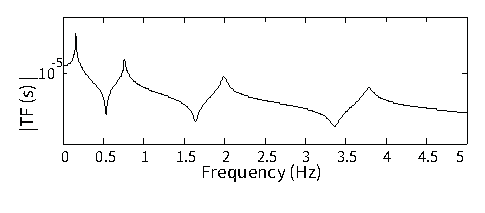
\includegraphics[width=0.8\textwidth] {figure/6-4b.eps}
   \label{fig:6-4b}
 }
\caption{Transfer function of 75th story responses to LMS.}
\label{fig:6-4}
\end{figure}

Figure~\ref{fig:6-5} shows the frequency response function and the time history of the actuator force obtained without using a filter when the target response is acceleration or displacement of the 75th floor. It is known from Figure~\ref{fig:6-5} that much larger force are required for the shaker to achieve the target displacement than acceleration response, and furthermore there exist high-frequency components in Figure~\ref{fig:6-4b}, which result in high-speed switching of control force as shown in Figure~\ref{fig:6-5b}. In practice, hydraulic actuators popular in civil engineering structures is not suitable for this undesirable chattering problem which causes spillover instability in higher modes, and acceleration response concerned with serviceability criteria is more critical for such high-rise building excited by wind load as this benchmark building than displacement. 
Figure~\ref{fig:6-6} shows the comparison between the frequency responses of wind and LMS induced 75th-floor acceleration and displacement when the target response is 75th displacement. It is obviously shown that the wind and LMD induced displacement coincide well with each other while acceleration responses are very different. Based upon the observation in Figure~\ref{fig:6-5} and  \ref{fig:6-6}, only acceleration response is considered as target response for calculating LMD force reproducing wind induced displacement as well as acceleration in this study.

\begin{figure}[!ht]
\centering
\subfigure[LMS force targeting on 75th floor acceleration.]{
   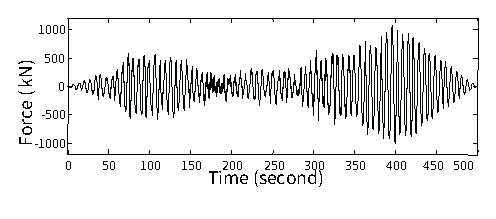
\includegraphics[width=0.8\textwidth] {figure/6-5a.eps}
   \label{fig:6-5a}
 }
 \subfigure[LMS force targeting on 75th floor displacement.]{
   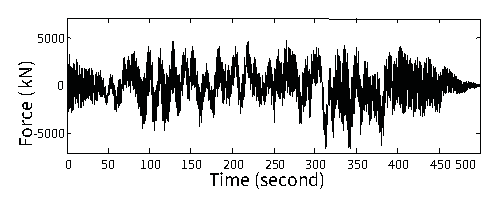
\includegraphics[width=0.8\textwidth] {figure/6-5b.eps}
   \label{fig:6-5b}
 }
\caption{LMS force (unfiltered).}
\label{fig:6-5}
\end{figure}

\begin{figure}[!ht]
\centering
\subfigure[Acceleration response.]{
   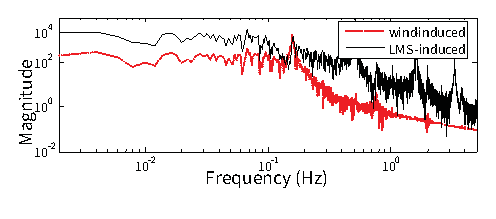
\includegraphics[width=0.8\textwidth] {figure/6-6a.eps}
   \label{fig:6-6a}
 }
 \subfigure[Displacement response.]{
   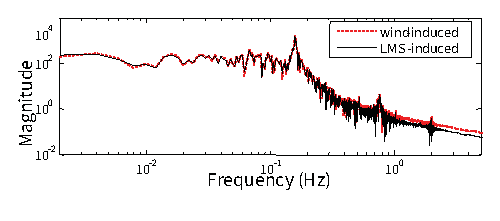
\includegraphics[width=0.8\textwidth] {figure/6-6b.eps}
   \label{fig:6-6b}
 }
\caption{Frequency response of 75th floor with LMD force targeting displacement response.}
\label{fig:6-6}
\end{figure}

Numerical analyses are conducted with/without using the filter and envelope function for different target responses. Table~\ref{tab:6-1} lists the cut-off frequencies used for canceling previously mentioned undesirable amplification effect by the zero in the inverse transfer function of each target response. Envelope function with $t_{1}=100$ second and $t_{2}=100$ second is applied.

\begin{table}[ht]
\centering
\begin{tabularx}{\textwidth}{@{}X|X|X@{}}
\toprule[1pt]\midrule[0.3pt]
Target response & $\omega_{1}$ (rad/sec) & $\omega_{2}$ (rad/sec)\\ \hline
75th floor acceleration & 1.01 & 1.13\\
50th floor acceleration & 8.17 & 8.80\\
30th floor acceleration & 17.59 & 20.73\\
\bottomrule
\end{tabularx}
\caption{Cutoff frequency for filter design}
\label{tab:6-1}
\end{table}

Figure~\ref{fig:6-7} shows the floor distribution of the time and frequency domain errors defined in the previous subsection, which are obtained with/without using the filter for different target responses. Processed signal denotes one yielded by using the filter. It is identified from Figure~\ref{fig:6-7} that the processed signal using filter significantly reduce the magnitude of the tracking error when the target response is 75-floor acceleration of which transfer function has band-stop frequency near the first modal frequency (as observed in Figure~\ref{fig:6-4a}) while the processing effect is trivial when the target response is 30th or 50th floor acceleration of which transfer function has zero away from the first modal one. Also, it is known from observing the error distribution that the targeted responses are almost identical to wind-induced ones with a small magnitude of error while the other non-targeted responses are slightly different with increasing error. Targeting 30th or 50th-floor acceleration provides greater discrepancy between the wind and LMS induced 75-floor accelerations which are critical in evaluating serviceability.
The comparison between the results in Figure~\ref{fig:6-7a} and \ref{fig:6-7b} indicates that the distribution tendency of $e_{t}$ and $e_{f}$ is quite different and the magnitude of $e_{t}$ is much larger than that of $e_{f}$. When targeting response is 75th floor acceleration, both values of $e_{t}$ and $e_{f}$ are smallest for the targeted 75th floor acceleration, but the value of $e_{f}$ becomes larger for the other story responses while the value of $e_{f}$ generally keeps the smallest except for 30th story acceleration. The larger value of $e_{t}$ results from the phase difference between the wind and LMS induced responses since $e_{t}$ is obtained based on the response difference at the same time step. The phase of the wind-induced response is not the important parameter in evaluating the wind resistance performance of a building structure, $e_{f}$ can be said to be the more appropriate index for evaluating the wind response reproducing the performance of LMS.

\begin{figure}[!ht]
\centering
\subfigure[$e_{t}$]{
   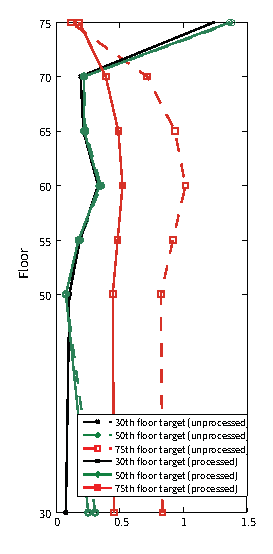
\includegraphics[width=0.45\textwidth] {figure/6-7a.eps}
   \label{fig:6-7a}\hfill
 }
 \subfigure[$e_{f}$]{
   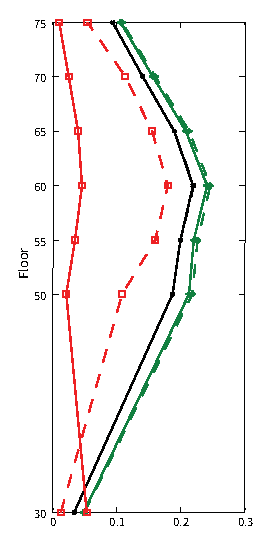
\includegraphics[width=0.45\textwidth] {figure/6-7b.eps}
   \label{fig:6-7b}
 }
\caption{Error distribution according to the filter usage and floor of target response.}
\label{fig:6-7}
\end{figure}

Figures~\ref{fig:6-8} and \ref{fig:6-9} compare the time histories of the wind and LMS induced structural responses for the cases that the target responses are, respectively, 75th and 30th-floor accelerations and filter are applied for the design of LMS. Figure~\ref{fig:6-8} shows that the LMS induced acceleration response including targeted 75th-floor acceleration agree well with wind-induced ones while displacement responses at all floors are underestimated by LMS. It is observed in Figure~\ref{fig:6-9} that the shaker simulated targeted 30th-floor acceleration as well as displacement responses but overestimates 75th-floor acceleration.

\begin{figure}[!ht]
\centering
\subfigure[76th story acceleration response]{
   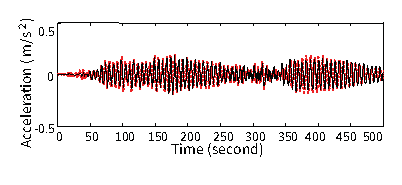
\includegraphics[width=0.45\textwidth] {figure/6-8a.eps}
   \label{fig:6-8a}\hfill
 }
 \subfigure[76th story displacement response]{
   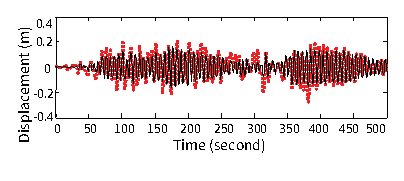
\includegraphics[width=0.45\textwidth] {figure/6-8b.eps}
   \label{fig:6-8b}
 }
 \subfigure[50th story acceleration response]{
   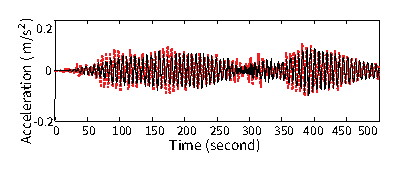
\includegraphics[width=0.45\textwidth] {figure/6-8c.eps}
   \label{fig:6-8c}\hfill
 }
 \subfigure[50th story displacement response]{
   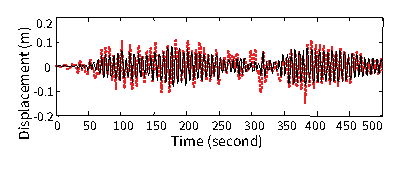
\includegraphics[width=0.45\textwidth] {figure/6-8d.eps}
   \label{fig:6-8d}
 }
 \subfigure[30th story acceleration response]{
   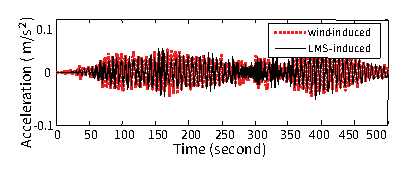
\includegraphics[width=0.45\textwidth] {figure/6-8e.eps}
   \label{fig:6-8e}\hfill
 }
 \subfigure[30th story displacement response]{
   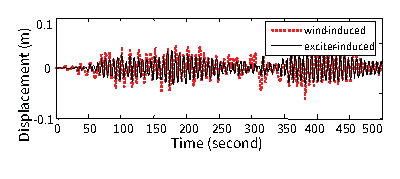
\includegraphics[width=0.45\textwidth] {figure/6-8f.eps}
   \label{fig:6-8f}
 }
\caption{Wind and LMS induced acceleration responses (when the target is 75th floor acceleration).}
\label{fig:6-8}
\end{figure}

\begin{figure}[!ht]
\centering
\subfigure[76th story acceleration response]{
   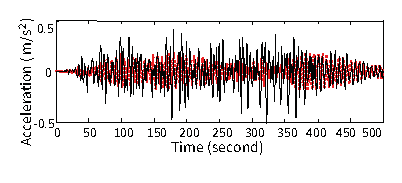
\includegraphics[width=0.45\textwidth] {figure/6-9a.eps}
   \label{fig:6-9a}\hfill
 }
 \subfigure[76th story displacement response]{
   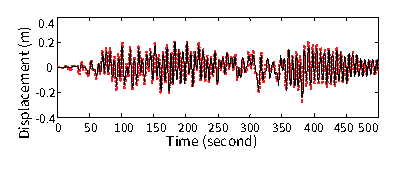
\includegraphics[width=0.45\textwidth] {figure/6-9b.eps}
   \label{fig:6-9b}
 }
 \subfigure[50th story acceleration response]{
   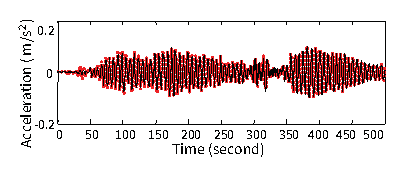
\includegraphics[width=0.45\textwidth] {figure/6-9c.eps}
   \label{fig:6-9c}\hfill
 }
 \subfigure[50th story displacement response]{
   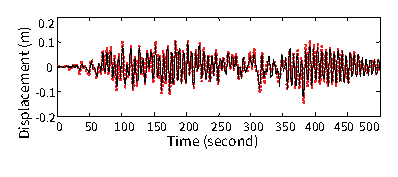
\includegraphics[width=0.45\textwidth] {figure/6-9d.eps}
   \label{fig:6-9d}
 }
 \subfigure[30th story acceleration response]{
   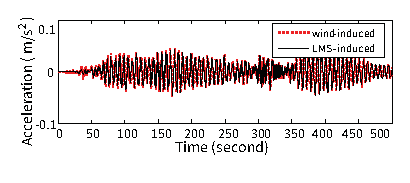
\includegraphics[width=0.45\textwidth] {figure/6-9e.eps}
   \label{fig:6-9e}\hfill
 }
 \subfigure[30th story displacement response]{
   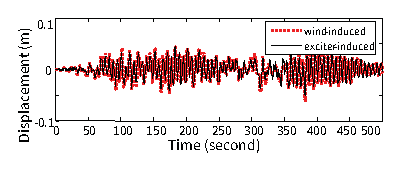
\includegraphics[width=0.45\textwidth] {figure/6-9f.eps}
   \label{fig:6-9f}
 }
\caption{Wind and LMS induced acceleration responses (when the target is 30th floor acceleration).}
\label{fig:6-9}
\end{figure}

\subsection{ATMD excitation}

In the 76th story building benchmark problem, ATMD is used as an example controller, which is composed of spring and viscous damper in addition to the mass and actuator of the LMS. In this subsection, the ATMD is considered as another exciter. The mass of the ATMD is 500 metric ton, and the undamped natural frequency and damping ratio are, respectively, 0.16Hz and 20\%\citep{yang2004benchmark}. Simplification for the control environments have been made, in particular, the actuator dynamics and controller-structure interaction are not considered in the benchmark problem. 
The equation of motion of the building equipped with an ATMD on the top floor can be expressed as

\begin{equation}\label{eq:6-10}
\matr{M}\matr{\ddot{x}}+\matr{C}\matr{\dot{x}}+\matr{K}\matr{x}+\matr{H}u = \eta\matr{W}
\end{equation}

and considering no wind-load input, the equation of motion of the building can be expressed as

\begin{equation}\label{eq:6-11}
\begin{aligned}
\begin{bmatrix}\matr{M}_{s} & 0 \\ \matr{0} & m_{t}\end{bmatrix}
\begin{psmatrix}\matr{\ddot{x}}_{s} \\ \ddot{x}_{t}\end{psmatrix}+&
\begin{bmatrix}\matr{C}_{s}+c_{t}\matr{B}_{t}\matr{B}_{t}^{\top} & -c_{t}\matr{B}_{t} \\ -c_{t}\matr{B}_{t}^{\top} & c_{t}\end{bmatrix}
\begin{psmatrix}\matr{\dot{x}}_{s} \\ \dot{x}_{t}\end{psmatrix}+\\
&\begin{bmatrix}\matr{K}_{s}+k_{t}\matr{B}_{t}\matr{B}_{t}^{\top} & -k_{t}\matr{B}_{t} \\ -k_{t}\matr{B}_{t}^{\top} & k_{t}\end{bmatrix}
\begin{psmatrix}\matr{x}_{s} \\ x_{t}\end{psmatrix}  =
\begin{bmatrix}-\matr{B}_{t}\\1 \end{bmatrix}u
\end{aligned}
\end{equation}

where $\matr{B}_{t}$ is position vector of floor installed ATMD, $\matr{M}_{s}$, $\matr{C}_{s}$ and $\matr{K}_{s}$ is the mass, damping coefficient and stiffness matrix of the structure and $m_{t}$, $c_{t}$ and $k_{t}$ is the mass, damping coefficient and stiffness of the ATMD. 

Figure~\ref{fig:6-10a} shows the transfer function of the 75th-floor acceleration to the absolute acceleration the ATMD. No zero point is observed in the vicinity of the first modal frequency unlike the case for LMS, which indicates that band-stop filter is not required for preventing the ATMD to excite the unexpected frequency response. Figure~\ref{fig:6-10b} shows the frequency response of the actuator force of the ATMD and Figure~\ref{fig:6-10c} and \ref{fig:6-10d} show the frequency and time responses of the effective force applied to the structure by the ATMD.

\begin{figure}[!ht]
\centering
\subfigure[Transfer function of ATMD induced structure]{
   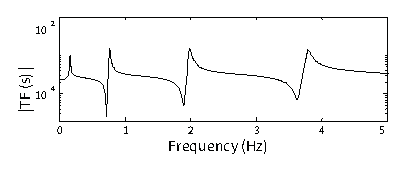
\includegraphics[width=0.45\textwidth] {figure/6-10a.eps}
   \label{fig:6-10a}\hfill
 }
 \subfigure[Frequency response of ATMD acceleration]{
   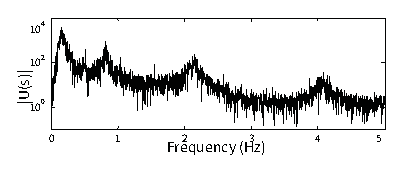
\includegraphics[width=0.45\textwidth] {figure/6-10b.eps}
   \label{fig:6-10b}
 }
 \subfigure[Frequency response of ATMD actuator force]{
   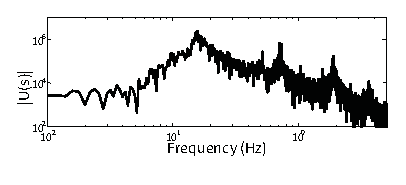
\includegraphics[width=0.45\textwidth] {figure/6-10c.eps}
   \label{fig:6-10c}\hfill
 }
 \subfigure[Time history of ATMD actuator force]{
   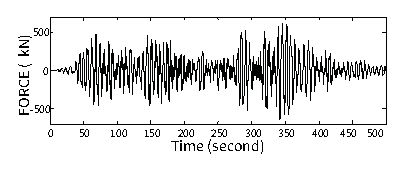
\includegraphics[width=0.45\textwidth] {figure/6-10d.eps}
   \label{fig:6-10d}
 }
\caption{ATMD Excitation.}
\label{fig:6-10}
\end{figure}

Figure~\ref{fig:6-11} shows the time history comparison between wind induced acceleration and ATMD induced one targeting on 75th story acceleration response.

All acceleration responses coincide well with each other, but in displacement response, there exists slight underestimation and overestimation according to the time ranges.

\begin{figure}[!ht]
\centering
\subfigure[76th story acceleration response]{
   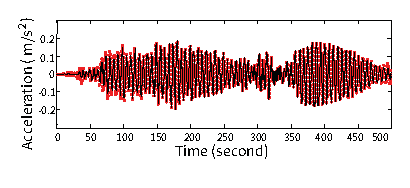
\includegraphics[width=0.45\textwidth] {figure/6-11a.eps}
   \label{fig:6-11a}\hfill
 }
 \subfigure[76th story displacement response]{
   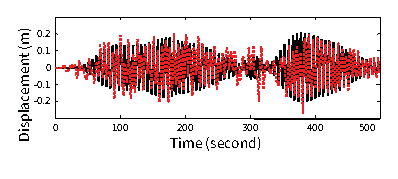
\includegraphics[width=0.45\textwidth] {figure/6-11b.eps}
   \label{fig:6-11b}
 }
 \subfigure[50th story acceleration response]{
   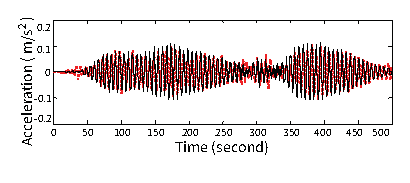
\includegraphics[width=0.45\textwidth] {figure/6-11c.eps}
   \label{fig:6-11c}\hfill
 }
 \subfigure[50th story displacement response]{
   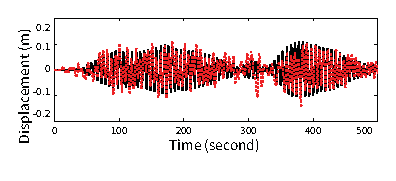
\includegraphics[width=0.45\textwidth] {figure/6-11d.eps}
   \label{fig:6-11d}
 }
 \subfigure[30th story acceleration response]{
   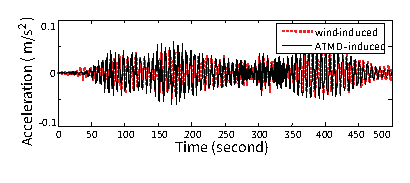
\includegraphics[width=0.45\textwidth] {figure/6-11e.eps}
   \label{fig:6-11e}\hfill
 }
 \subfigure[30th story displacement response]{
   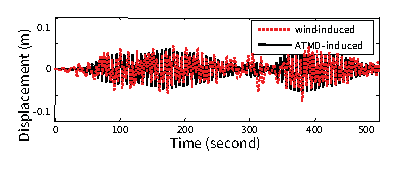
\includegraphics[width=0.45\textwidth] {figure/6-11f.eps}
   \label{fig:6-11f}
 }
\caption{Wind and ATMD induced acceleration responses (when the target is 75th floor acceleration).}
\label{fig:6-11}
\end{figure}

Figure~\ref{fig:6-12} shows the comparison between the frequency responses of 75th floor acceleration and it is observed that wind and ATMD induced responses show good agreement over all frequency range. 

\begin{figure}[ht]
\centering
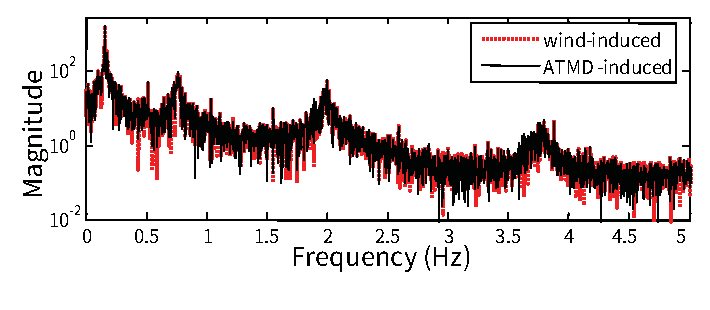
\includegraphics[width=0.8\textwidth] {figure/6-12.eps}
\caption{Frequency response of wind and ATMD induced 75th floor accelerations}
\label{fig:6-12}
\end{figure}

Figure~\ref{fig:6-13} shows the error distribution according to the floor of targeted acceleration response. From Figure~\ref{fig:6-13b} showing that $e_{f}$ has the smallest value over floors when the target response is 75th floor acceleration, and the corresponding value ranges only between 1\% and 10\%, ATMD targeting 75th floor acceleration can be said to provide the best performance, and it can exactly reproduce the wind-induced acceleration response of all floors including targeted 75th floor.

\begin{figure}[!ht]
\centering
\subfigure[$e_{t}$]{
   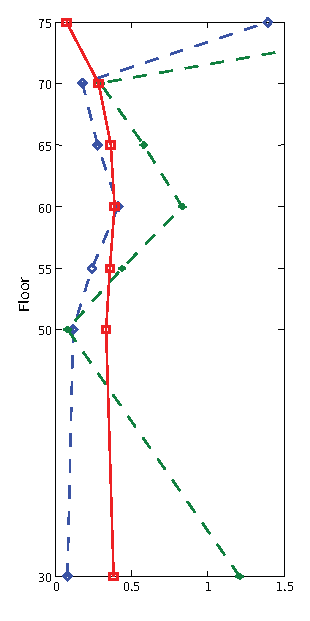
\includegraphics[width=0.45\textwidth] {figure/6-13a.eps}
   \label{fig:6-13a}\hfill
 }
 \subfigure[$e_{f}$]{
   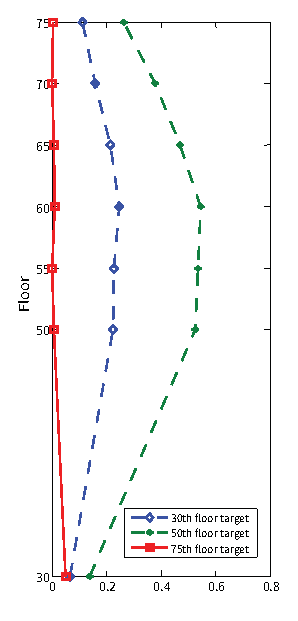
\includegraphics[width=0.45\textwidth] {figure/6-13b.eps}
   \label{fig:6-13b}
 }
\caption{Error Distribution with ATMD excitation.}
\label{fig:6-13}
\end{figure}

\subsection{Comparison between LMS and ATMD}

Figure~\ref{fig:6-14} shows time history of the actuator forces in LMS and ATMD excitation systems. The peak actuator force required for ATMD is larger than that for LMS. Figure~\ref{fig:6-15} compares the stroke of LMS with/without filter and ATMD. The stroke of LMS with filter is much smaller than those of LMS without filter and ATMD. This fact implies that ATMD requires large stroke to show good performance in wind-induced response realization and this stroke requirement should be checked in the design of ATMD.

\begin{figure}[ht]
\centering
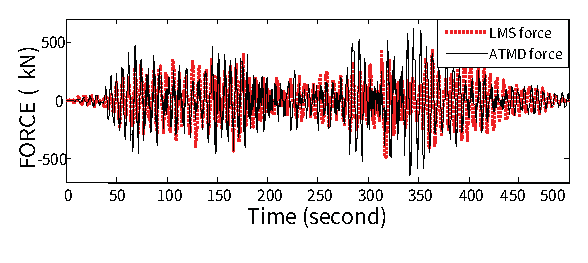
\includegraphics[width=0.8\textwidth] {figure/6-14.eps}
\caption{Comparison between actuator forces in LMS and ATMD}
\label{fig:6-14}
\end{figure}

\begin{figure}[!ht]
\centering
\subfigure[LMS stroke (unfiltered)]{
   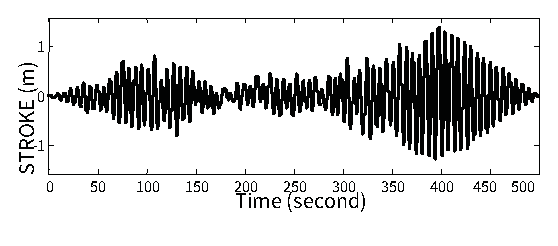
\includegraphics[width=0.8\textwidth] {figure/6-15a.eps}
   \label{fig:6-15a}
 }
 \subfigure[LMS stroke (filtered)]{
   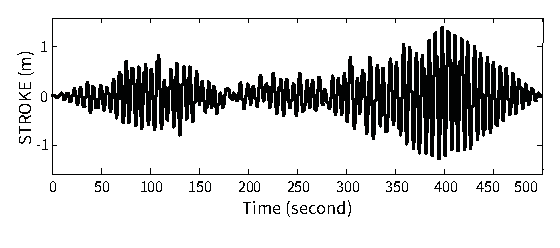
\includegraphics[width=0.8\textwidth] {figure/6-15b.eps}
   \label{fig:6-15b}
 }
 \subfigure[ATMD stroke]{
   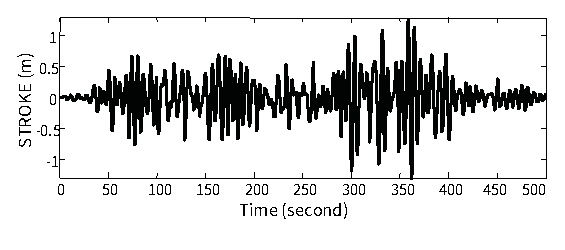
\includegraphics[width=0.8\textwidth] {figure/6-15c.eps}
   \label{fig:6-15c}
 }
\caption{Stroke Comparison.}
\label{fig:6-15}
\end{figure}

Table~\ref{tab:6-2} shows the numerical values of the error, actuator force, and actuator stroke in LMS with/without the filter, and ATMD systems. The errors are obtained when the target and evaluation responses are identical, and actuator force and stroke are obtained when the target response is 75th-floor acceleration. The facts observed from Figures~\ref{fig:6-14} and \ref{fig:6-15} that the performance of LMS can be enhanced using the band-stop filter and ATMD reproduces wind-induced response better than LMS, but ATMD requires larger actuator force and stroke can be identified once more.

\begin{table}[ht]
\centering
\begin{tabularx}{\textwidth}{@{}XX|X|X|X@{}}
\toprule[1pt]\midrule[0.3pt]
&& LMS (unfiltered) & LMS (filtered) & ATMD \\ \hline
75th floor acceleration & $e_{t}$ & 0.117 & 0.192 & 0.074 \\
& $e_{f}$ & 0.054 & 0.011 & 0.003 \\ \hline
50th floor acceleration & $e_{t}$ & 0.081 & 0.081 & 0.083 \\
& $e_{f}$ & 0.219 & 0.213 & 0.525 \\ \hline
30th floor acceleration & $e_{t}$ & 0.082 & 0.082 & 0.082 \\
& $e_{f}$ & 0.034 & 0.033 & 0.065 \\ \hline
Stroke & Peak (m) & 1.402 & 0.519 & 1.265 \\
& RMS (m) & 0.436 & 0.183 & 0.333 \\ \hline
Actuator force & Peak (kN) & 1068.22 & 441.68 & 655.78 \\
& RMS (kN) & 323.92 & 136.44 & 170.39 \\
\bottomrule
\end{tabularx}
\caption{Comparison between LMS and ATMD}
\label{tab:6-2}
\end{table}

\subsection{Summary}
The design of excitation systems for simulating wind-induced responses of a building structure was presented as a preliminary study for evaluating wind-resistance characteristics of building structures. The actuator forces of the LMS and ATMD were obtained using the inverse transfer function of structural responses. Also, band stop filter was used in LMS to remove zero of the transfer function such that undesirable modal excitation is prevented and envelop function was used to reduce the error occurring in transient initial states in both LMS and ATMD. The numerical analyses results from a 76-story benchmark building confirmed that the structural responses of a building structure excited by wind loads acting at all floors could be reproduced by the proposed excitation systems installed at a specific floor. The performances of the excitation systems were dependent on type and position of the target structural response for which acceleration response was suitable because targeting displacement response required large and high-speed changing control force.






%!TEX encoding = UTF-8 Unicode
\section{Forced vibration test of full-scaled five-story building structure simulating eqarthquake responses}
\label{chap:7}
\subsection{Overview}


In this section, the hybrid mass damper (HMD) controller for the pseudo-earthquake excitation test is designed by employing the method using the inverse transfer function of a structure, which is one of the methodologies proposed by the previous section and is verified for its experimental implementation. First, a real scaled five-story steel frame, in which an HMD installed, is shaken and then transfer functions from the HMD to structural responses of each story are obtained. Then, the FE model numerically calculated from the software for commercial use is renewed based on the modal information extracted from experimentally obtained transfer functions. Also, the earthquake responses based on the renewed structural model are numerically calculated, and the structure is excited by an HMD input signal which is produced to simulate a specific target response of a structure out of these numerically calculated earthquake responses. Finally, the effectiveness of pseudo-earthquake excitation presented in this study is verified by comparing numerically calculated seismic responses with experimentally measured ones.

The pseudo-earthquake excitation testing method presented in this study has a few importance in an engineering aspect. First, the testing method that is performed for a real scale structure in the field is free from lots of artificial constraints accompanied in a laboratory test. Secondly, valuable data, which are available for the verification of structural seismic performance and the evaluation of the availability of vibration technique required in structural health monitoring, can be acquired from the test. Thirdly, large shaking table is not required to evaluate the seismic response of real-scaled building structures, since in this study the earthquake response is simulated by actuating a structure with an HMD installed at the upper story.

\subsection{Experimental Real-Scale Building Model}
The experimental model, which is shown in Figures~\ref{fig:7-1} and \ref{fig:7-2}, is a full-scale five-story steel structure which has the story height of 6m, the plan of $6m\times6m$, and the story mass of 20,000kg. Each floor is composed of four identical wide-flange type steel columns. An HMD using larger scale linear motor damper which was also designed as a passive damper has a moving mass on the fifth floor excited the model structure. Because the columns consist of I-shaped steel, the HMD was installed in minor axis of the structure.

\begin{figure}[!ht]
\centering
\subfigure[minor axis]{
   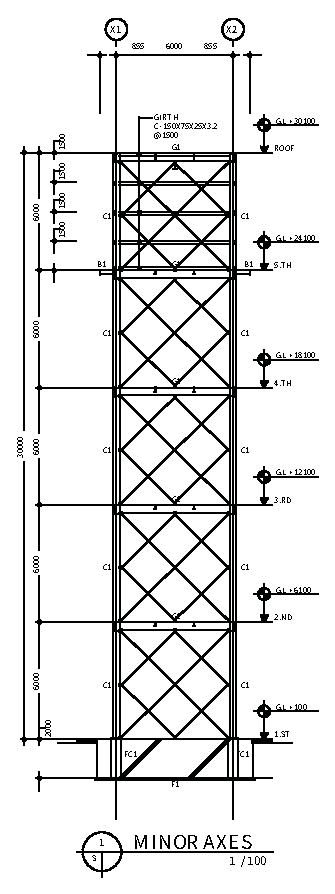
\includegraphics[width=0.45\textwidth] {figure/7-1a.eps}
   \label{fig:7-1a}\hfill
 }
 \subfigure[major axis]{
   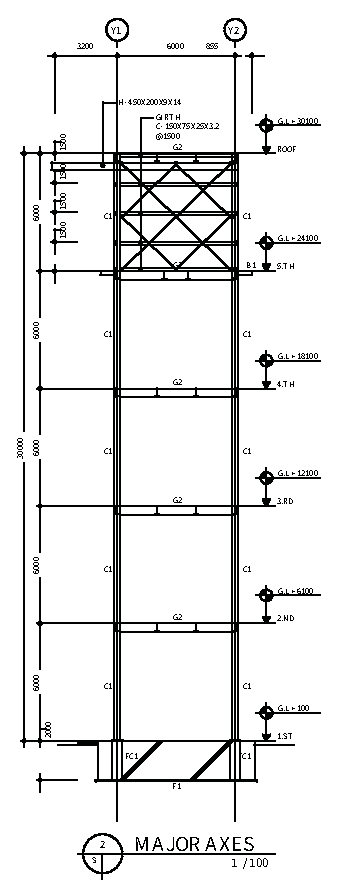
\includegraphics[width=0.45\textwidth] {figure/7-1b.eps}
   \label{fig:7-1b}
 }
\caption{Elevation view of the target structure.}
\label{fig:7-1}
\end{figure}

\begin{figure}[!ht]
\centering
\subfigure[Five-story building structure.]{
   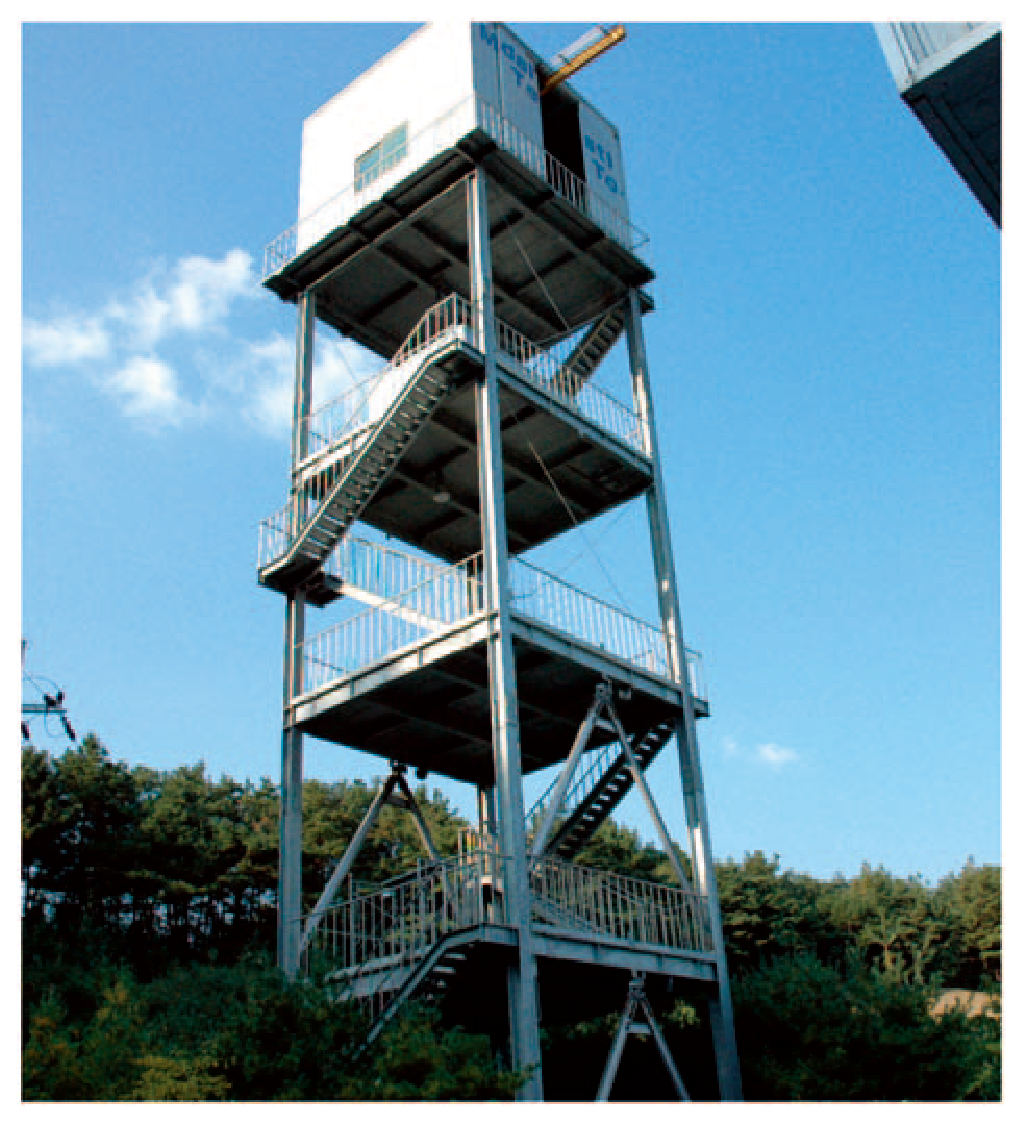
\includegraphics[width=0.45\textwidth] {figure/8-4.eps}
   \label{fig:7-1a}\hfill
 }
 \subfigure[Transfer function of target floor response to the HMD.]{
   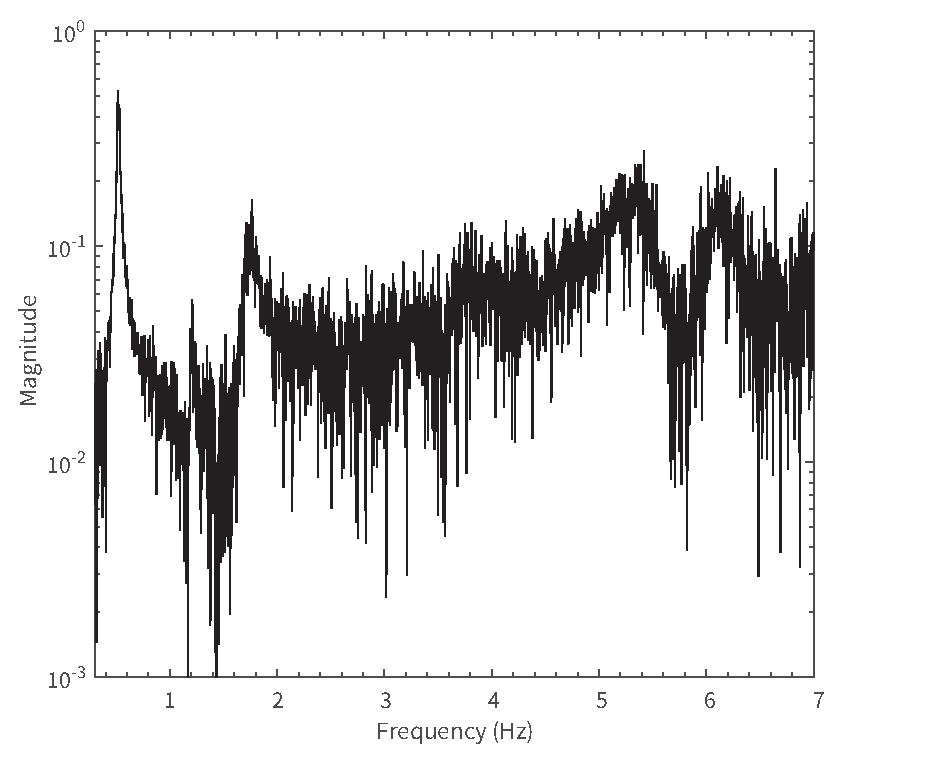
\includegraphics[width=0.45\textwidth] {figure/7-2b.eps}
   \label{fig:7-1b}
 }
\caption{Photograph and transfer function of the target building structure.}
\label{fig:7-2}
\end{figure}

\begin{table}[ht]
\centering
\begin{tabularx}{\textwidth}{s|b}
\toprule[1pt]\midrule[0.3pt]
\multicolumn{2}{c}{MEMBER LIST}\\ \midrule[0.3pt]
C1&H-310$\times$310$\times$20$\times$20\\
G1&H-400$\times$200$\times$8$\times$13\\
G2&H-450$\times$200$\times$9$\times$14\\
B1&H-200$\times$100$\times$5.5$\times$8\\
B2&H-400$\times$200$\times$8$\times$13\\
RB1&H-400$\times$200$\times$8$\times$13\\
FC1&500$\times$500\\
\bottomrule
\end{tabularx}
\caption{Member list of the model structure}
\label{tab:7-1}
\end{table}

\subsection{Field measurement and experimental system}
Field measurement and experimental system is shown in Figures~\ref{fig:7-3} and \ref{fig:7-4}. In order to minimize the latency between the excitation and the measurement, one lap-top PC in the experimental system was used for simultaneously implementing the excitation and the measurement. The measurement system has accelerometers, PCB Corp. 393B12 model was installed at the center of the 2nd~5th floor and KYOWA Corp. AS-2GB model was attached to the HMD. PCB Monitran and KYOWA DPM-711B was used to amplify their measured signals. The data cabling connection system has BNC cable with lengths of 25m and 50m. In the data acquisition system, the DAQ board of NI DAQCard-6036E with 16bit-range was used to perform the AD and DA conversion. Also, it was connected to the signal conditioner of NI SCC-2345 by using both the input modules and the output module. 
In this excitation system, both excitation and measurement signals are voltage signals, and this excitation signal transfers equivalent thrust generated according to the input voltage signal through the inverter of HMD, to the mass of HMD. Accordingly, the excitation signal should be generated to move within the safety range, because the excessive response of the HMD is prevented by its safety device.

\begin{figure}[ht]
\centering
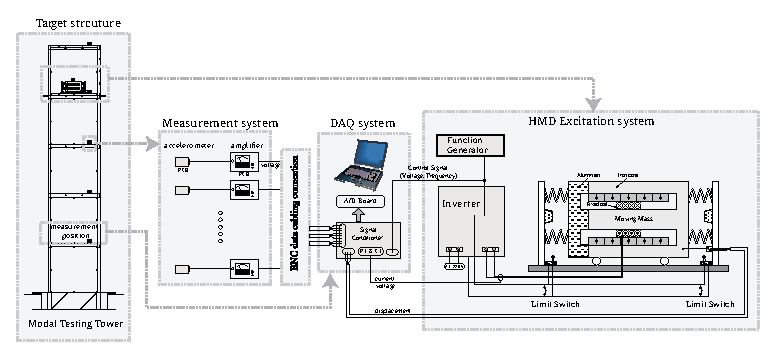
\includegraphics[width=1\textwidth] {figure/7-3.eps}
\caption{Schematic diagram of the field measurement, data acquisition and excitation system.}
\label{fig:7-3}
\end{figure}

\begin{figure}[!ht]
\centering
\subfigure[The measurement and data acquisition system]{
   \includegraphics[width=0.45\textwidth] {figure/7-4a.eps}
   \label{fig:7-4a}\hfill
 }
 \subfigure[The accelerometer installation]{
   \includegraphics[width=0.45\textwidth] {figure/7-4b.eps}
   \label{fig:7-4b}
 }
\caption{Installation pictures of the measurement, data acquisition and excitation system.}
\label{fig:7-4}
\end{figure}

\subsection{System Identification}
\subsubsection{White-noise Test}
White noise vibration test was carried out by using broad-band random signals during 410sec. Both the excitation and measurement were performed by constructing a close-loop system to minimize the latency, by which time delay would be induced, and experimental data was acquired with a sampling rate of 100Hz. In order to reduce the unexpected noise in the experiment, a low-pass filter of 30Hz within the amplifier and 25Hz within the signal conditioner module was utilized, and the acquisition system was insulated with the reference signal ended (RSE) method for its grounding.
Figure~\ref{fig:7-5} shows the transfer function from the absolute acceleration of the HMD to the building accelerations. The lower fundamental modes of the structure are apparently shown.

\begin{figure}[ht]
\centering
\includegraphics[width=1\textwidth] {figure/7-5.eps}
\caption{The transfer function from the absolute acceleration of the HMD to those of the structure.}
\label{fig:7-5}
\end{figure}

% \subsubsection{Modal parameter identification methods}
% \subsubsubsection{Frequency domain methods}
% The peak picking (PP) method using power spectral density (PSD) function is widely used in practice\citep{bendat1980engineering}. \citet{bao1991determination} proposed the three types of mode shape using power spectral density function as

% \begin{equation}\label{eq:7-1}
% \phi_{ak}^{(I)} = \frac{\hat{S}_{y_{a}y_{b}}(f_{k})}{\hat{S}_{y_{b}y_{b}}(f_{k})},
% \phi_{ak}^{(II)} = \frac{\hat{S}_{y_{a}y_{a}}(f_{k})}{\hat{S}_{y_{a}y_{b}}(f_{k})},
% \phi_{ak}^{(III)} = sign\left(\phi_{ak}^{(I)}\right)\left\{\frac{\hat{S}_{y_{a}y_{b}}(f_{k})}{\hat{S}_{y_{b}y_{b}}(f_{k})}\right\}^{1/2}
% \end{equation}

% where, $f_{k}$ is $k$th natural frequency, and $S_{y_{a}y_{a}}$ and $S_{y_{a}y_{b}}$ are the auto-spectral density function and the cross-spectral density function, respectively. The relationship between three type of mode shape before normalizing can be obtained as\citep{feng1998identification}.

% \begin{equation}\label{eq:7-2}
% \begin{aligned}
% \phi_{ak}^{(I)} &\leq \phi_{ak} \leq \phi_{ak}^{(III)}\\
% \phi_{ak}^{(I)} &\leq \phi_{ak}^{(III)} \leq \phi_{ak}^{III}
% \end{aligned}
% \end{equation}
% where $\phi_{ak}$ is the true mode shape of the structure. The details for PP method about the mode shape with type (I) in Eq.~\eqref{eq:7-1} are described in the Appendix. A.

% It is frequently address that it is very difficult or impossible to identify closely spaced mode using the PP. In this case, the frequency domain decomposigion (FDD) method that utilizes the singular value decomposition of the PSD matrix may be used to separate close modes\citep{brinker2000modal}. The method was originally used to extract the operational deflection shapes in mechanical vibrating systems\citep{otte1990operational}. The natural frequencies are estimated from the peaks of the PSD functions in the PP method. On the other hand, they are evaluated from singular value (SV) functions of the PSD matrix in the FDD method.

% \begin{equation}\label{eq:7-3}
% \matr{S}_{yy}(\omega) = \matr{U}(\omega)\matr{s}(\omega)\matr{V}(\omega)^{\top}
% \end{equation}

% where $\matr{S}_{yy}(\omega) \in \mathbb{R}^{Nm\times Nm}$ is the PSD matrix for output responses $\matr{y}(t) \in \mathbb{R}^{Nm}$, $\matr{s}(\omega) \in \mathbb{R}^{Nm \times Nm}$ is a diagonal matrix containing the singular values of its PSD matrix, and $\matr{U}(\omega)$, $\matr{V}(\omega) \in \mathbb{R}^{Nm \times Nm}$ are corresponding unitary matrices. $Nm$ is the number of measuring points. The general multi-DOF system can be transformed to the single DOF shape can be estimated as the first column vector of the unitary matrix of $\matr{U}$ since the first singular value may include the structural mode nearby its natural frequencies. However in the closely spaced modes, the peak of largest singular values at one natural frequency indicate the structural mode and adjacent second singular value mey indicate the close mode.

% \subsubsubsection{Time domain methods}
% The Ibrahim time domain (ITD) and the eigensystem realization algorithm (ERA) methods were originally formulated using the free decaying signals. However, to deal with the responsed to random excitations, they were extened to the ITD/RD (random decremental technique) by employing randomdec signature\citep{ibrahim1977method} and to the ERA/DC (data correlation) by using cross-correlation function\citep{juang1994applied}. Generally, the randomdec signal and the cross-correlation function are similar to free decaying signals. In this study, the ITD employing cross-correlation function, namely ITD/DC, is introduced since the processing time to obtain the randomdec signature is generally much more than that of cross-correlation function. The background to use cross-correlation function as an alternative of free decaying signal is described in the Appendix B. A column of the correlation matrix associated with a reference point is used in the ITD/DC, while the whole matrix may be processed in the ERA/DC. The stochasting subspace identification (SSI) method utilizing the Hankel matrix of the correlation function block\citep{van2012subspace} can be classifed into the SSI-BR (balanced realization) and the SSI-CVA(canonical variate analysis) depending on the construction method of the Hankel amtrix\citep{hermans1999modal}. It is very interesting to note that the SSI/BI is basically same to the ERA/DC except for the realization step. It is very important to detemine the optimal model order in the ERA and the SSI methods. There are several approaches to select the optimal model order. However, the stabilization chart may be very stable modes can be determined. Figure 2.2 and Table~\ref{tab:7-2} show the stabilization chart and the estimated results for Unison Modal Tower by using the SSI/BR method. In the stabilization chart, there are three identified modes: noise mode, unstable mode, and stable mode. In this study, the noise modes were classified by using the damping ratio greater than 50\%, and the stable modes are determined that the comparisons of the several mode with small frequency difference(0.5\% in this study), and high modal assurance criteria\citep{ewins1984modal} value (0.99 in this study). The reesult are compared with the peaks of the first singular values by FDD method. It can be clearly observed that the stable modes are located at the peak in the FDD plot.

\begin{table}[ht]
\centering
\begin{tabularx}{\textwidth}{s|b|b}
\toprule[1pt]\midrule[0.3pt]
Modes & Frequency (Hz) \& COV (\%) & Damping ratio (\%) \& COV (\%)\\ \midrule[0.3pt]
1&0.52(1.82) & 1.46(14.42)\\
2&1.73(0.13) & 2.71(9.40)\\
3&2.94(0.10) & 3.54(1.93)\\
4&4.14(0.08) & 1.72(1.70)\\
5&5.36(0.23) & 3.84(3.56)\\
\bottomrule
\end{tabularx}
\caption{Identified natural frequencies and damping ratios}
\label{tab:7-2}
\end{table}

\subsubsubsection{Finite Model Updating}
It is difficult to establish the FE model because of limitations in the number of sensors that may be deployed and the difficulty of actuating a structure to higher modes. The process of developing an FE model of a structure relating it to the experimental model is called FE model updating\citep{bagchi2005updating}. In this paper, an analysis model was established by modeling using ANSYS and model updating was carried out by using the measured modal data.

In this paper, the optimal matrix update method was used which is based on a constraint optimization problem where the minimum changes in the mass matrix or the stiffness matrix are found subject to constraints such as symmetry, connectivity, and definiteness\citep{baruch1978optimization, baruch1979optimal}. The mass matrix is assumed to be exact. There exists a constraint on the corrected stiffness matrix which should reproduce the measured modal data with symmetry. The two independent constraint equations are Eqs.~\eqref{eq:7-4} and \eqref{eq:7-5}. The function to be minimized must relate in some way to the difference between the corrected stiffness matrix, $\matr{K}$, and the analytically derived stiffness matrix, $\matr{K}_{a}$, which is shown in the form of the norm in Eq.~\eqref{eq:7-6}. The expression for the updated mode and stiffness matrix, which is obtained by minimizing Eq.~\eqref{eq:7-6} satisfying Eqs.~\eqref{eq:7-4} and \eqref{eq:7-5}, lead to Eqs.~\eqref{eq:7-7} and \eqref{eq:7-8}\citep{baruch1979optimal, baruch1978optimization}.

\begin{equation}\label{eq:7-4}
\matr{K}\Phi = \matr{M}_{a}\Phi\Lambda, \Phi^{\top}\matr{M}_{a}\Phi = \matr{I}
\end{equation}

\begin{equation}\label{eq:7-5}
\matr{K}^{\top} = \matr{K}
\end{equation}

\begin{equation}\label{eq:7-6}
J=\frac{1}{2}\left\| \matr{N}^{-1}\left(\matr{K}-\matr{K}_{a}\right)^{-1}\right\|
\end{equation}

\begin{equation}\label{eq:7-7}
\Phi = \Phi_{m} \left[ \Phi_{m}^{\top}\matr{M}_{a}\Phi_{m}\right]^{-1/2}
\end{equation}

\begin{equation}\label{eq:7-8}
\begin{aligned}
\matr{K}&=\matr{K}_{a} - \matr{K}_{a}\Phi\Phi^{\top}\matr{M}_{a}-\matr{M}_{a}\Phi\Phi^{\top}\matr{K}_{a}\\
&+\matr{M}_{a}\Phi\Phi^{\top}\matr{K}_{a}\Phi\Phi^{\top}\matr{M}_{a} + \matr{M}_{a}\Phi\Lambda\Phi^{\top}\matr{M}_{a}
\end{aligned}
\end{equation}

where, $\matr{M}_{a}$ and $\matr{K}_{a}$ are the analytically derived mass matrix and stiffness matrix, respectively, $\Phi_{m}$ is the measured eigenvector matrix, $\Lambda$ is a diagonal matrix of the measured eigenvalues and $\matr{N}$ is the appearance of the square root of the mass matrix $\matr{N} = \matr{M}_{a}^{1/2}$.

In this study, as shown in Figure~\ref{fig:7-5}, the measured eigenvector is extracted from the measured modal data using respectively accurate the first and the second modal information. When the measured eigenvector matrix would be extracted, it could be extracted from the transfer function in case of modal resonance using Eq.~\eqref{eq:7-9} and the sign of the eigenvector are determined from the phase of the transfer function. Reinhorn et al. assumed that resonance responses of the each mode are dependent in case the modal frequencies are not adjacent each other and proposed equation of the transfer function, which is expressed as

\begin{equation} \label{eq:7-9}
T_{ai}\left(\omega_{k}\right) = \phi_{ik}H_{ik}\left(\omega_{k}\right)\Gamma_{k}
\end{equation}

where, $T_{ai}\left(\omega_{k}\right)$, $H_{ik}\left(\omega_{k}\right)$ are the transfer functions to the $i$th floor and the $k$th mode of structures in case of resonance and not, $\Gamma_{k}$ is the $k$th scalar value of $\Gamma = -\Phi^{\top}\matr{M}_{a}\matr{I}$ and $\matr{I}$ is the influence vector of HMD load. The $k$th value of eigenvector by ratio of the $i$th floor over the $j$th floor can be calculated from amplitude ratio of the transfer function to absolute acceleration responses, which is expressed as

\begin{equation}\label{eq:7-10}
\phi_{ik}/\phi_{jk} = T_{ai}\left(\omega_{k}\right)/T_{aj}\left(\omega_{k}\right)
\end{equation}

\begin{table}[ht]
\centering
\begin{tabularx}{\textwidth}{@{}X|X|X|X|X|X@{}}
\toprule[1pt]\midrule[0.3pt]
& 1st mode & 2nd mode & 3rd mode & 4th mode & 5th mode\\ \midrule[0.3pt]
initial & 0.5022 & 1.5623 & 2.74 & 3.91 & 4.83\\
measured& 0.5249 & 1.7578 & 2.94 & 3.67 & 5.38\\
updated & 0.5249 & 1.7578 & 2.95 & 3.67 & 5.38\\
\bottomrule
\end{tabularx}
\caption{Natural frequencies (Hz) for the modal testing tower}
\label{tab:7-3}
\end{table}

By updating the natural frequencies and modes, the exact results are obtained comparing to those of the initial analysis.

\begin{figure}[!ht]
\centering
\subfigure[1st mode shape]{
   \includegraphics[width=0.45\textwidth] {figure/7-6a.eps}
   \label{fig:7-6a}\hfill
 }
 \subfigure[2nd mode shape]{
   \includegraphics[width=0.45\textwidth] {figure/7-6b.eps}
   \label{fig:7-6b}
 }
\caption{The mode shape comparison of initial, the measured and the updated FE models.}
\label{fig:7-6}
\end{figure}

\begin{figure}[!ht]
\centering
\subfigure[Transfer function of HMD to 1st floor acceleration]{
   \includegraphics[width=0.6\textwidth] {figure/7-7a.eps}
   \label{fig:7-7a}\hfill
}
\subfigure[Transfer function of HMD to 2nd floor acceleration]{
   \includegraphics[width=0.6\textwidth] {figure/7-7b.eps}
   \label{fig:7-7b}
}
\subfigure[Transfer function of HMD to 3rd floor acceleration]{
   \includegraphics[width=0.6\textwidth] {figure/7-7c.eps}
   \label{fig:7-7c}\hfill
}
\subfigure[Transfer function of HMD to 4th floor acceleration]{
   \includegraphics[width=0.6\textwidth] {figure/7-7d.eps}
   \label{fig:7-7d}
}
\subfigure[Transfer function of HMD to 5th floor acceleration]{
   \includegraphics[width=0.6\textwidth] {figure/7-7e.eps}
   \label{fig:7-7e}
}
\caption{The transfer function comparison of the initial, measured, updated FE model.}
\label{fig:7-7}
\end{figure}

\subsection{Design Controller of an Excitation System for Simulating Earthquake Response}
\subsubsection{Generating Input Signal of HMD}\label{sec:7-5-1}
In this chapter, the process of generating the HMD input signal which is simulating earthquake response in the elastic range of model structure by HMD is introduced. The state-space form equation of a structure excited by the base acceleration $\ddot{u}_{b}$ and HMD acceleration $\ddot{u}_{h}$ with size of $r$ is expressed as follows

\begin{equation}\label{eq:7-11}
\begin{aligned}
\matr{\dot{z}}&= \matr{A}\matr{z} + \matr{B}_{b}\ddot{u}_{b}+\matr{B}_{h}\ddot{u}_{h}\\
\matr{y}&=\matr{C}\matr{z}+\matr{D}_{b}\ddot{u}_{b}+\matr{D}_{h}\ddot{u}_{h}
\end{aligned}
\end{equation}

where $\matr{z}$ is state variable vector size of $2n\times1$ and $\matr{y}$ is output vector with size of $m$. The output transfer functions to $\ddot{u}_{b}$ or $\ddot{u}_{h}$ are given by

\begin{equation}\label{eq:7-12}
\begin{aligned}
\matr{T}_{h}&=\matr{Y}_{h}(s)\matr{U}_{h}(s)^{-1} = \matr{C}\left(s\matr{I}-\matr{A}\right)^{-1}\matr{B}_{h} + \matr{D}_{h}\\
\matr{T}_{b}&=\matr{Y}_{b}(s)\matr{U}_{b}(s)^{-1} = \matr{C}\left(s\matr{I}-\matr{A}\right)^{-1}\matr{B}_{b}
\end{aligned}
\end{equation}

where the scalar $s$ is a complex variable $j\omega$. The inverse of $\matr{T}_{h}$ exists only if $r$ equals to $m$ and the Laplace transform of $\ddot{u}_{h}$ providing the identical output to the base acceleration induced one is detemined as

\begin{equation}\label{eq:7-13}
\matr{U}_{h}(s) = \matr{T}_{h}^{-1}\matr{Y}_{h}(s) = \matr{T}_{h}^{-1}\matr{Y}_{b}(s) = \matr{T}_{h}^{-1}\matr{T}_{b}\matr{U}_{b}(s)
\end{equation}

when $r$ is smaller than $m$, the number of structural responses which can be modulated by $\ddot{u}_{h}$ is restricted to $r$ and target structural response should be selected. The Laplace transform of input realizing the target response $\bar{y}$ with size of $r$ is

\begin{equation}\label{eq:7-14}
\hat{U}_{h}(s) = \hat{T}_{h}^{-1}\hat{Y}_{h}(s) = \hat{T}_{h}^{-1}\hat{Y}_{b}(s) = \hat{T}_{h}^{-1}\hat{T}_{b}\hat{U}_{b}(s)
\end{equation}

where, $\hat{T}_{h}^{-1}$ is a sub-matrices of $\matr{T}_{h}^{-1}$. $\hat{T}_{h}^{-1}$ is constructed by extracting the columns in $\matr{T}_{h}^{-1}$ corresponding to the target response.

\subsubsection{Design of HMD controller}\label{sec:7-5-2}
The excitation force is generated by the HMD to vibrate the structure in the elastic range. In order to control the HMD, the linear oscillating actuator (LOA) using electromagnetic force as an exciter was adopted. The mass of HMD is 1,500kg mass mounted in the 5th floor of the structure. The excitation force is generated by not the HMD acceleration of input voltage signal but 5th-floor absolute acceleration. Therefore, in order to compensate the distortion of the actual HMD acceleration against the HMD dynamics existing between the reference signal and the actual measured acceleration of the HMD, the inverse transfer function of the actual acceleration of HMD with respect to the command signal generated by the control computer is constructed and implemented in the HMD control computer as shown in Figure~\ref{fig:7-9}. First, the inverse transfer function, of which amplitude and phase are represented in Figure~\ref{fig:7-10} by the dashed line, is obtained experimentally. Then, the experimental inverse transfer function is approximated by a rational function for its implementation in the control computer. In this verification experiment, the inverse transfer function of the HMD is approximated using the command \code{invfreqs} in MATLAB\citep{coleman1999optimization}, which adopts the damped Gauss-Newton method for iterative search to minimize the sum of the squared error between the measured and the desired frequency response points\citep{dennis1983numerical}. The approximation result is given by the following linear filter and compared with the experimental one in Figure~\ref{fig:7-10}.

\begin{figure}[ht]
\centering
\includegraphics[width=0.8\textwidth] {figure/7-8.eps}
\caption{Photograph of the HMD installed in 5th floor.}
\label{fig:7-8}
\end{figure}

\begin{figure}[!ht]
\centering
\subfigure[Definition of the transfer function of the HMD]{
   \includegraphics[width=0.8\textwidth] {figure/7-9a.eps}
   \label{fig:7-9a}\hfill
 }
 \subfigure[Compensation the dynamics of HMD using the inverse transfer function]{
   \includegraphics[width=0.8\textwidth] {figure/7-9b.eps}
   \label{fig:7-9b}
 }
\caption{Schematic diagram of the HMD controller.}
\label{fig:7-9}
\end{figure}

\begin{figure}[!ht]
\centering
\subfigure[Magnitude]{
   \includegraphics[width=0.8\textwidth] {figure/7-10a.eps}
   \label{fig:7-10a}\hfill
 }
 \subfigure[Phase]{
   \includegraphics[width=0.8\textwidth] {figure/7-10b.eps}
   \label{fig:7-10b}
 }
\caption{Comparison of the measured and the approximated inverse transfer function of the HMD.}
\label{fig:7-10}
\end{figure}

\begin{figure}[!ht]
\centering
\subfigure[Acceleration of HMD excited by El Centro earthquake]{
   \includegraphics[width=0.8\textwidth] {figure/7-11a.eps}
   \label{fig:7-11a}\hfill
 }
 \subfigure[Acceleration of HMD excited by Hachinohe earthquake]{
   \includegraphics[width=0.8\textwidth] {figure/7-11b.eps}
   \label{fig:7-11b}
 }
\caption{Comparison of the reference and measured acceleration time histories when the signals were generated by El Centro and Hachinohe earthquake.}
\label{fig:7-11}
\end{figure}

\subsection{Experimental results}
\subsubsection{Pseudo-earthquake excitation result}
The pseudo-earthquake forced vibration testing is implemented. The earthquake El Centro(1940, NS) and Hachinohe(1968, NS) earthquake acceleration which PGAs were scaled down to 0.05g for the safety limit device were used in this study. The pseudo-earthquake excitation signal was generated by the inverse transfer function of structure introduced in the chapter~\ref{sec:7-5-1} corresponding to the target responses and the excitation was implemented through the HMD controller introduced in the chapter~\ref{sec:7-5-2}.

Figure~\ref{fig:7-12} compares the result in time history of El Centro earthquake response in the analysis and experimental models. It is observed that both results from FE model and experimental one coincides well each other in the initial time range, but the phase in post time range shows a tendency to be changed over 90 degrees. It is caused that the constraint in curve fitting the transfer function was considered weightily with the amplitude of the response, not the phase since in the seismic performance of the structure the amplitude was laid more weight on than the phase.

\begin{figure}[!ht]
\centering
\subfigure[1st floor acceleration of El Centro earthquake excitation]{
   \includegraphics[width=0.45\textwidth] {figure/7-12a.eps}
   \label{fig:7-12a}\hfill
}
\subfigure[2nd floor acceleration of El Centro earthquake excitation]{
   \includegraphics[width=0.45\textwidth] {figure/7-12b.eps}
   \label{fig:7-12b}
}
\subfigure[3rd floor acceleration of El Centro earthquake excitation]{
   \includegraphics[width=0.45\textwidth] {figure/7-12c.eps}
   \label{fig:7-12c}\hfill
}
\subfigure[4th floor acceleration of El Centro earthquake excitation]{
   \includegraphics[width=0.45\textwidth] {figure/7-12d.eps}
   \label{fig:7-12d}
}
\subfigure[5th floor acceleration of El Centro earthquake excitation]{
   \includegraphics[width=0.45\textwidth] {figure/7-12e.eps}
   \label{fig:7-12e}\hfill
}
\subfigure[1st floor displacement of El Centro earthquake excitation]{
   \includegraphics[width=0.45\textwidth] {figure/7-12f.eps}
   \label{fig:7-12f}
}
\caption{Time history comparison of El Centro earthquake response in the analysis and experimental models. (when the target response is the 5th-floor acceleration).}
\label{fig:7-12}
\end{figure}

Figure~\ref{fig:7-13} compares the result in the frequency domain of El Centro earthquake response in analysis model and experimental one. It is observed that both of results from FE model and experimental one coincides well each other, respectively

\begin{figure}[!ht]
\centering
\subfigure[1st floor acceleration response]{
   \includegraphics[width=0.45\textwidth] {figure/7-13a.eps}
   \label{fig:7-13a}\hfill
}
\subfigure[2nd floor acceleration response]{
   \includegraphics[width=0.45\textwidth] {figure/7-13b.eps}
   \label{fig:7-13b}
}
\subfigure[3rd floor acceleration response]{
   \includegraphics[width=0.45\textwidth] {figure/7-13c.eps}
   \label{fig:7-13c}\hfill
}
\subfigure[4th floor acceleration response]{
   \includegraphics[width=0.45\textwidth] {figure/7-13d.eps}
   \label{fig:7-13d}
}
\subfigure[5th floor acceleration response]{
   \includegraphics[width=0.45\textwidth] {figure/7-13e.eps}
   \label{fig:7-13e}\hfill
}
\subfigure[1st floor displacement response]{
   \includegraphics[width=0.45\textwidth] {figure/7-13f.eps}
   \label{fig:7-13f}
}
\caption{Comparison in frequency domain of El Centro earthquake response of the analysis and experimental models. (when the target response is the 5th floor acceleration).}
\label{fig:7-13}
\end{figure}

Figure~\ref{fig:7-14} compares the result in the time domain of Hachinohe earthquake response in analysis model and experimental one. It is observed that both of results from FE model and experimental one are good agreement and demonstrate the effectiveness proposed pseudo-earthquake forced vibration testing method. The discrepancy in amplitude at the second mode frequency is caused by the difficulty of excitation a structure to higher modes limits the modal testing method to capturing only a few lower modes. In order to improve this phenomenon, it should be designed to be able to excite higher mode which has fundamental frequencies of a structure.

\begin{figure}[!ht]
\centering
\subfigure[1st floor acceleration of Hachinohe earthquake excitation]{
   \includegraphics[width=0.45\textwidth] {figure/7-14a.eps}
   \label{fig:7-14a}\hfill
}
\subfigure[2nd floor acceleration of Hachinohe earthquake excitation]{
   \includegraphics[width=0.45\textwidth] {figure/7-14b.eps}
   \label{fig:7-14b}
}
\subfigure[3rd floor acceleration of Hachinohe earthquake excitation]{
   \includegraphics[width=0.45\textwidth] {figure/7-14c.eps}
   \label{fig:7-14c}\hfill
}
\subfigure[4th floor acceleration of Hachinohe earthquake excitation]{
   \includegraphics[width=0.45\textwidth] {figure/7-14d.eps}
   \label{fig:7-14d}
}
\subfigure[5th floor acceleration of Hachinohe earthquake excitation]{
   \includegraphics[width=0.45\textwidth] {figure/7-14e.eps}
   \label{fig:7-14e}\hfill
}
\subfigure[1st floor displacement of Hachinohe earthquake excitation]{
   \includegraphics[width=0.45\textwidth] {figure/7-14f.eps}
   \label{fig:7-14f}
}
\caption{Time history comparison of Hachinohe earthquake response in the analysis and experimental models. (when the target response is the 5th-floor acceleration).}
\label{fig:7-14}
\end{figure}

Figure~\ref{fig:7-15} compares the result in the frequency domain of Hachinohe earthquake response in analysis model and experimental one. It is observed that the coincidence of the response at the first mode and second mode frequency was shown, but it would not reflect the responses at the third mode or higher mode frequency in Figures~\ref{fig:7-15a}-\ref{fig:7-15c}.

\begin{figure}[!ht]
\centering
\subfigure[1st floor acceleration response]{
   \includegraphics[width=0.45\textwidth] {figure/7-15a.eps}
   \label{fig:7-15a}\hfill
}
\subfigure[2nd floor acceleration response]{
   \includegraphics[width=0.45\textwidth] {figure/7-15b.eps}
   \label{fig:7-15b}
}
\subfigure[3rd floor acceleration response]{
   \includegraphics[width=0.45\textwidth] {figure/7-15c.eps}
   \label{fig:7-15c}\hfill
}
\subfigure[4th floor acceleration response]{
   \includegraphics[width=0.45\textwidth] {figure/7-15d.eps}
   \label{fig:7-15d}
}
\subfigure[5th floor acceleration response]{
   \includegraphics[width=0.45\textwidth] {figure/7-15e.eps}
   \label{fig:7-15e}\hfill
}
\subfigure[1st floor displacement response]{
   \includegraphics[width=0.45\textwidth] {figure/7-15f.eps}
   \label{fig:7-15f}
}
\caption{Comparison in frequency domain of Hachinohe earthquake response in the analysis and experimental models. (when the target response is the 5th-floor acceleration).}
\label{fig:7-15}
\end{figure}

\subsection{Error Analysis}

The normalized RMS error between the absolute acceleration induced by HMD and the base acceleration could be express as Eq.~\eqref{eq:7-15}. Figure~\ref{fig:7-16} is shown the floor distribute errors corresponding to the target responses of the analysis FE model. All responses are contained 10-20\% error values and the minimal error value presented when the target response consider the 5th-floor acceleration.

\begin{equation}\label{eq:7-15}
\text{Normalized RMS Error(\%) } \epsilon = \frac{\sum_{t=0}^{T}\left\{\sqrt{\ddot{y}_{g}(t)^{2}}\right\} - \sum_{t=0}^{T}\left\{\sqrt{\ddot{y}_{h}(t)^{2}}\right\}}{\sum_{t=0}^{T}\left\{\sqrt{\ddot{y}_{g}(t)^{2}}\right\}}
\end{equation}

where $\ddot{y}_{g}$, $\ddot{y}_{h}$ are the structural acceleration responses which are the base acceleration and the HMD acceleration induced. $T$ is total excitation time of the earthquakes.

\begin{figure}[!ht]
\centering
\subfigure[El Centro]{
   \includegraphics[width=0.4\textwidth] {figure/7-16a.eps}
   \label{fig:7-16a}\hfill
 }
 \subfigure[Hachinohe]{
   \includegraphics[width=0.4\textwidth] {figure/7-16b.eps}
   \label{fig:7-16b}
 }
\caption{Normalized RMS error floor distribution of the analysis FE model corresponding the distributed floor acceleration response.}
\label{fig:7-16}
\end{figure}

Figure~\ref{fig:7-17} shows the floor distribute errors of the experimentally measured response corresponding to the target responses. All responses are contained 20-30\% error values when the HMD induced.

\begin{figure}[!ht]
\centering
\subfigure[El Centro]{
   \includegraphics[width=0.4\textwidth] {figure/7-17a.eps}
   \label{fig:7-17a}\hfill
 }
 \subfigure[Hachinohe]{
   \includegraphics[width=0.4\textwidth] {figure/7-17b.eps}
   \label{fig:7-17b}
 }
\caption{Normalized RMS error floor distribution of the experimental results corresponding the distributed floor acceleration response.}
\label{fig:7-17}
\end{figure}

\subsection{Summary}
In this section, field measurement system of a full-scale structure and excitation system were established and then forced vibration test was carried out using the HMD to simulate seismic load. System identification of the full-scale structure was carried out through white noise test, and finite element model is updated. The seismic excitation system was accomplished through inverse transfer functions of structure and HMD by the system identifications. The propriety of seismic excitation system was verified by a comparison between the seismic numerical analysis results of finite element model and the experimental results of HMD excitation.



\section{Forced vibration test of MR Damper-based Semiactive Control Algorithms for Full-scaled Building}
\label{chap:expmr}
\subsection{Overview}

In this section, the effectiveness of the MR damper-based semiactive control systems for seismic protection of a full-scale five-story steel frame building structure is experimentally verified, when some semi-active control algorithms such as the clipped-optimal control algorithm (CO), the maximum energy dissipation algorithm (MEDA), the Lyapunov stability theory based control algorithm (LYAP) and the neuro-control algorithm are considered. This may be the first experimental investigation of several semi-active control algorithms using a full-scale test structure. In the experiment, two MR dampers are attached between the ground and the first floor. As described in the previous section, the pseudo-earthquake testing method is used to excite the building structure as if it is subjected to earthquake loading. This method uses filters that modify the displacement of the HMD using both transfer function in the frequency domain and the least squares approximation in the time domain. All the semi-active control algorithms are evaluated under four historical earthquakes (El Centro, Hachinohe, Kobe, and Northridge earthquakes) and one filtered artificial earthquake. The experimental results are compared with the passive optimal case which provides the specific constant voltage to the MR damper.


\subsection{Full scaled MR Damper}
\citet{lee2010experimental} had developed full-scale MR damper, an MR damper is designed by deriving a suboptimal design procedure considering optimization problem and magnetic analysis, and a damper with the capacity of 1.0ton is manufactured.

\begin{table}[ht]
\centering
\begin{tabularx}{\textwidth}{@{}X|X|X|X@{}}
\toprule[1pt]\midrule[0.3pt]
No. of stage & 3 & 3 & 4\\ \hline
Flux density in steel & $<$ 1.5T & $>$ 1.5T & $<$ 1.5T\\
Magnetic field intensity & $<$ 150 kAmp/m  & $>$150 kAmp/m  & $<$ 150 kAmp/m \\
Coil turns & 20AWG/200 turns  & 20AWG/230 turns & 21AWG/200 turns  \\
Input current & 3A  & 3A & 3A  \\
\bottomrule
\end{tabularx}
\caption{Results obtained from the magnetic analysis.}
\label{tab:n3-1}
\end{table}

In order to use the designed MR dampers in the experiment, two MR dampers are manufactured as shown in Figure~\ref{fig:n3-6a} and~\ref{fig:n3-6b} and tested with harmonic dynamic displacements applied by a servo-hydraulic testing system. The result of variable current tests is shown in Figure~\ref{fig:n3-6c}. As shown in Figure~\ref{fig:n3-6c}, the total damper force at design velocity (60mm/s) is about 10kN. Among the total force, the uncontrollable force is about 2kN or more and controllable force approximately 8kN or less.

\begin{figure}[!ht]
\centering
\subfigure[Components of full scaled MR Damper]{
   \includegraphics[width=0.4\textwidth] {figure/n3-6a.eps}
   \label{fig:n3-6a}\hfill
}
\subfigure[Manufactured full scaled MR Damper]{
   \includegraphics[width=0.4\textwidth] {figure/n3-6b.eps}
   \label{fig:n3-6b}
}
\subfigure[Variable current test]{
   \includegraphics[width=0.6\textwidth] {figure/n3-6c.eps}
   \label{fig:n3-6c}\hfill
}

\caption{Manufactured MR damper and test result.}
\label{fig:n3-6}
\end{figure}

\subsection{Semi-active control algorithms}

Semi-active control algorithms determine the most appropriate voltage to change viscous characteristics of the MR damper from the structural response measurements. Since the MR damper force is related to not only command voltage but also the relative velocity and displacement between both ends of the damper, the MR dampers cannot be directly controlled by the command voltage. So far various semi-active control algorithms have been proposed for control of MR dampers~\citep{jansen2000semiactive}. In this section, four different control algorithms are considered; CO, LYAP, MEDA, and cost function-based SNC.

\subsection{External excitation loads}
In order to evaluate the performance of the MR damper-based semi-active control algorithms and passive control system, a suite of historical ground motions that are intended to encompass both moderate events and severe events is considered as external excitation load. Moreover, a filtered artificial earthquake (Kanai-Tajimi filter) is also adopted to verify the effectiveness of the control algorithms. Each historical ground motion and the artificial earthquake are scaled down in order to bound HMD by limited maximum displacement for safety. Each ground motions used in this investigation are as follows and the acceleration of HMD and its power spectral density are shown in Figure~\ref{fig:n3-10-1} and \ref{fig:n3-10-2}.

\subsubsection{Moderate events}
\begin{itemize}
\item El Centro : N-S component of the 1940 Imperial valley, California earthquake (magnitude 7.1) recorded at Imperial Valley Irrigation District substation in El Centro, California, USA (scaled down to 0.303g);
\item Hachinohe : N-S component of the 1968 Takochioki(Hachinohe) earthquake (magnitude 7.9) recorded at Hachinohe, Japan (scaled down to 0.265g);
\end{itemize}

\subsubsection{Severe events}
\begin{itemize}
   \item Kobe : N-S component of the 1995 Hyogo-ken Nanbu(Kobe) earthquake (magnitude 7.2) recorded at Kobe Japanese Meteorological Agency (JMA), Kobe, Japan (scaled down to 0.318g);

   \item  Northridge : N-S component of the 1994 Northridge earthquake (magnitude 6.8) recorded at the Sylmarcounty Hospital parking lot in Sylmar, California, USA (scaled down to 0.227g);
\end{itemize}

\subsubsection{Artificial eartuquake}
\begin{itemize}
   \item  Kanai-Tajimi filtered artificial earthquake (PGA:0.105g)
\end{itemize}

\begin{figure}[!ht]
\centering
\subfigure[Scaled El Centro earthquake]{
   \includegraphics[width=0.40\textwidth] {figure/n3-10a-1.eps}
   \label{fig:n3-10a-1}\hfill
   \includegraphics[width=0.43\textwidth] {figure/n3-10a-2.eps}
   \label{fig:n3-10a-2}
}
\subfigure[Scaled Hachinohe earthquake]{
   \includegraphics[width=0.40\textwidth] {figure/n3-10b-1.eps}
   \label{fig:n3-10b-1}\hfill
   \includegraphics[width=0.43\textwidth] {figure/n3-10b-2.eps}
   \label{fig:n3-10b-2}
}
\subfigure[Scaled Kobe earthquake]{
   \includegraphics[width=0.40\textwidth] {figure/n3-10c-1.eps}
   \label{fig:n3-10c-1}\hfill
   \includegraphics[width=0.43\textwidth] {figure/n3-10c-2.eps}
   \label{fig:n3-10c-2}
}
\caption{Acceleration of HMD and PSD used as external excitation load.}
\label{fig:n3-10-1}
\end{figure}

\begin{figure}[!ht]
\subfigure[Scaled Northridge earthquake]{
   \includegraphics[width=0.40\textwidth] {figure/n3-10d-1.eps}
   \label{fig:n3-10d-1}\hfill
   \includegraphics[width=0.43\textwidth] {figure/n3-10d-2.eps}
   \label{fig:n3-10d-2}
}
\subfigure[Kanai-Tajimi filtered artificial earthquake]{
   \includegraphics[width=0.40\textwidth] {figure/n3-10e-1.eps}
   \label{fig:n3-10e-1}\hfill
   \includegraphics[width=0.43\textwidth] {figure/n3-10e-2.eps}
   \label{fig:n3-10e-2}
}
\caption{Acceleration of HMD and PSD used as external excitation load.}
\label{fig:n3-10-2}
\end{figure}

\subsection{Measurement Devices and Feedback Control System}

Measurement devices used in this experiment are displacement sensors, accelerometers, load cells, and a current probe. The displacement sensors are used in measuring the relative displacement between ground and the first floor, which is the displacement of MR damper’s both ends. When the MR dampers are installed, two LVDT type potentiometers (Midori America LP-19FB) are used. To the contrary, two laser displacement sensors (Optex CD4-350D) are used, when the MR dampers are not installed. Each floor’s acceleration is measured by five accelerometers (PCB 393A03) and that of LAMD by Kyowa AS-2GB accelerometer. The load cells (CAS load cell LS-2T) measuring the MR damper control force are installed between the MR damper and the first floor. The current probes (Tektronix A622) measuring the current into each MR damper are also installed along the MR damper’s power cable.

The measured data from the above measurement devices are collected and digitalized through a data acquisition system (NI DAQ-card 6062E). The collected data is selected for each semi-active control algorithm, and finally, determined command voltage is sent to a current generator, which converts the voltage to the corresponding current. Then the MR damper can control the building structure with the generated current.

Finally, the MR damper controlled semi-active feedback system, which has 12 inputs and two outputs, can be formed as shown in Figure~\ref{fig:n3-11}.

\begin{figure}[!ht]
\centering
\includegraphics[width=0.50\textwidth] {figure/n3-11.eps}
\label{fig:n3-11}
\caption{MR damper-based semi-active feed back control system.}
\end{figure}

The CO, as well as the cost function-based SNC algorithm, needs full state or the particular state of the structural system to calculate the appropriate desired control force. The control implementation requires full number of sensors for all DOFs. Therefore the Kalman filters as an observer for state estimation is desirable. Considered a controllable and observable system and assumed that full state estimation is required. Then the primary purpose of the general Kalman filter is constructing a state estimate $\hat{\mathbf{x}}(t)$ that minimizes the steady-state error  covariance which is defined by:

\begin{equation}\label{eq:n3-13}
P = \lim_{t\to\infty} E\left(\left[ \mathbf{x} - \hat{\mathbf{x}} \right] \left[ \mathbf{x} - \hat{\mathbf{x}} \right]^{\top}\right)
\end{equation}

The optimal estimator for the state of interest is the Kalman filter which can be expressed as:

\begin{equation}\label{eq:n3-14}
\begin{aligned}
\hat{\mathbf{x}} &= \left(\mathbf{A}-\mathbf{LC}\right)\hat{\mathbf{x}} + \begin{bmatrix}\mathbf{L} & \mathbf{B}-\mathbf{LD}\end{bmatrix} \begin{psmatrix}\mathbf{y}\\\mathbf{u}\end{psmatrix} \\
\begin{psmatrix}\hat{\mathbf{y}}\\\hat{\mathbf{x}}\end{psmatrix} & = \begin{bmatrix}\mathbf{C} \\ \mathbf{I}\end{bmatrix}\hat{\mathbf{x}} + \begin{bmatrix}\mathbf{0} & \mathbf{D}\\ \mathbf{0} & \mathbf{0}\end{bmatrix}\begin{psmatrix}y \\ \mathbf{u}\end{psmatrix}
\end{aligned}
\end{equation}

where filter gain $\mathbf{L}$  is determined by solving an algebraic Riccati equation. The Kalman filter uses the known input $\mathbf{u}$ and the measurements $\mathbf{y}$ to generate the output and state estimates, that is, $\hat{\mathbf{y}}$ and $\hat{\mathbf{x}}$. Note that $\hat{\mathbf{y}}$  estimates the true system output without
noises.

\subsection{Testing building model}

All the stories in this building are 6m in height and are $6\times6m^{2}$ in the plan. In order to investigate the modal characteristics of the building, a forced vibration test is performed using a hybrid mass damper (HMD) located on the fourth floor in the previous section. The building is excited by a white-noise signal with frequency components of 0-10 Hz, and the corresponding acceleration responses are then measured at each floor. Using these measured acceleration data, transfer functions in the frequency domain are obtained, as shown by the dotted lines in Figure~\ref{fig:7-7}. Finally, the structural damping and stiffness matrices are identified based on the experimentally obtained transfer functions, as shown by the solid lines in Figure~\ref{fig:7-7}. The estimated mass and the identified damping and stiffness matrices are given in Eqs.~\eqref{eq:8-5}-\eqref{eq:8-7}, respectively, with results of 0.52, 1.76, 2.95, 3.67, and 5.38 Hz for each mode.


\begin{align}
\matr{M}_{5} & = \begin{bmatrix} 19365.5 & 0 & 0 & 0 & 0\\ 0 & 19365.5 & 0 & 0 & 0 \\ 0 & 0 & 19365.5 & 0 & 0 \\ 0 & 0 & 0 & 19365.5 & 0 \\ 0 & 0 & 0 & 0 & 19365.5\end{bmatrix}kg \label{eq:8-5} \\
\matr{C}_{5} & = \begin{bmatrix} 14.184 & -5.015 & 0.084  & -0.789 & 0.101 \\ -5.015 & 14.990  & -6.397 & 0.822 & -1.145 \\ 0.084  & -6.397 & 15.830  & -6.120  & -0.925 \\ -0.789 & 0.822  & -6.120 & 14.065  & -6.383 \\ 0.101 & -1.145  & -0.925  & -6.383 & 9.750\end{bmatrix}kN\cdot s/m \label{eq:8-6} \\
\matr{K}_{5} & = \begin{bmatrix} 7473.953 & 4860.497 & 1295.606 & -908.262 & 432.162 \\ -4860.497 & 9640.722 & -6637.235 & 2446.225 & -926.951 \\ 1295.606 & -6637.235 & 10861.354 & -6005.863 & 748.607 \\ -908.262 & 2446.225 & -6005.863 & 9132.066 & -4852.783 \\ 432.162 & -926.951 & 748.607 & -4852.783 & 4543.854\end{bmatrix}kN\/m \label{eq:8-7}
\end{align}

% \clearpage
% \begin{figure}[H]
% \centering
% \subfigure[fifth floor]{
%    \includegraphics[width=0.6\textwidth] {figure/8-5a.eps}
%    \label{fig:8-5a}\hfill
% }
% \subfigure[fourth floor]{
%    \includegraphics[width=0.6\textwidth] {figure/8-5b.eps}
%    \label{fig:8-5b}
% }
% \subfigure[third floor]{
%    \includegraphics[width=0.6\textwidth] {figure/8-5c.eps}
%    \label{fig:8-5c}\hfill
% }
% \subfigure[second floor]{
%    \includegraphics[width=0.6\textwidth] {figure/8-5d.eps}
%    \label{fig:8-5d}
% }
% \subfigure[first floor]{
%    \includegraphics[width=0.6\textwidth] {figure/8-5e.eps}
%    \label{fig:8-5e}
% }
% \caption{Measured and identified transfer functions with the HMD acceleration (dotted line :experiment, solid lines: identification).}
% \label{fig:8-5}
% \end{figure}

\subsection{Experimental results}
The passive control cases which provide specific constant voltage or current to the MR damper are the simplest means to operate the semiactive control using MR damper, because they need neither control algorithms nor measuring sensors. In this paper, therefore, the passive optimal case is determined by a series of passively controlled experiments and compared with the performance of the other semi-active control algorithms.

\subsubsection{Optimal Passive Case}
As described above, passive control cases provide specific constant voltage or current to the MR damper. A passive-off case means a case of which voltage is always set to zero, and a passive-on case sets the voltage to the maximum level. Since the maximum current level of the manufactured MR damper used in the experiments is 3.0A, a series of passively controlled tests are conducted as increasing the current level from 0.0A to 3.0A by 0.5A to obtain the passive optimal case. Figures~\ref{fig:n3-12} and~\ref{fig:n3-13} show the normalized maximum displacement of the first floor and the normalized maximum acceleration among all the five floors. 

It is demonstrated from Figure~\ref{fig:n3-12} that the performance in the maximum displacement gets better as the current input is increased. The passive-off case (i.e., 0.0A current input) shows the worst performance. In addition, the passive control cases with 1.0 or larger input current show the similar performance. As seen in Figure~\ref{fig:n3-13}, however, there is no trend in the performance of the normalized maximum acceleration. Under the moderate earthquakes and the artificial earthquake, most of the normalized values in maximum acceleration beneath 1.0 which means that the controlled seismic response might be reduced compared with that of the uncontrolled case. Nevertheless, most of the normalized values in acceleration are larger than 1.0 under the severe earthquake such as Kobe and Northridge earthquake. These results indicate that the MR damper-based passive control system is more suitable in moderate earthquake region than severe earthquake region for reducing the structural acceleration. From the observation as mentioned above, the passive control case with 1.0A can be considered as the optimal passive case. The results in cases of the passive optimal (1.0A) and passive on (3.0A) cases are compared with those in the cases of the other semi-active control algorithms.

\begin{figure}[!ht]
\centering
\includegraphics[width=0.6\textwidth] {figure/n3-12.eps}
\caption{Normalized maximum displacement of passive control
cases (first floor).}
\label{fig:n3-12}
\end{figure}

\begin{figure}[!ht]
\centering
\includegraphics[width=0.6\textwidth] {figure/n3-13.eps}
\caption{Normalized maximum acceleration of passive control
cases.}
\label{fig:n3-13}
\end{figure}

\subsubsection{Semiactive Control Cases}

After the optimal passive case is determined, the full-scale five-story steel frame building structure is excited with previously mentioned external excitation loads using LAMD and controlled with various semi-active control algorithms, such as the clipped optimal control algorithm (CO), the LYAP, the MEDA, and the SNC, using MR dampers. The responses of each control case are measured and summarized in Figures~\ref{fig:n3-14} and~\ref{fig:n3-15}. Figure~\ref{fig:n3-14} shows the normalized maximum displacement of the first floor with various control algorithms and Figure~\ref{fig:n3-15} shows the normalized maximum acceleration among all the floors. From the experimental results, one can conclude as follows:

The CO shows good performance in reducing both displacement and acceleration. For severe earthquakes and artificial earthquake, however, the performance becomes slightly worse than that of moderate earthquakes. In order to obtain the better control performance from the CO, it should be designed more appropriately by altering the weighting parameters for the specific purpose of a designer. The Lyapunov algorithm and the SNC algorithm reduce the acceleration response well enough, but they cannot show the good performance in reducing displacement. In these cases, the MR dampers generate less control force than in the clipped optimal algorithm case. The Lyapunov algorithm shows the worst performance among five algorithms in reducing acceleration under the artificial earthquake, and the SNC has a drawback in reducing displacement under the severe earthquakes.
Note that among all the semi-active control algorithms, the MEDA shows the best performance in reducing displacement and the worst performance in reducing acceleration. As the MEDA makes the MR dampers generate larger force, the first floor is almost locked with the ground. This causes a considerable increase of the acceleration response of the first floor.
It is shown in some cases that maximum acceleration with the controller is larger than that of the uncontrolled case. It is considered that in the experiments, the unexpected electrical and the external environmental noises are involved in the feedback of measured responses, which deteriorates the acceleration control performance that is sensitive to those noises. The passive optimal and passive-on cases are one of the best control algorithms in reducing displacement of the structure except for the performance in reducing acceleration.
The inter-story drift between the first and second floors can be larger than the displacement of the first floor when the damper force is quite large. Due to the limitation in measuring displacements, the inter-story drift of the second floor could not be measured. In order to verify the above observation, the inter-story drift of the second floor should be measured in the additional tests. The LYAP and SNC algorithms are appropriate in reducing accelerations of the structural system. On the other hand, the passive optimal and passive-on cases and the MEDA show excellent performance in reducing the first-floor displacement.

\begin{figure}[!ht]
\centering
\includegraphics[width=0.6\textwidth] {figure/n3-14.eps}
\caption{Normalized maximum displacement comparison of MR damper-based control systems.}
\label{fig:n3-14}
\end{figure}

\begin{figure}[!ht]
\centering
\includegraphics[width=0.6\textwidth] {figure/n3-15.eps}
\caption{Normalized maximum acceleration comparison of MR damper-based control systems.}
\label{fig:n3-15}
\end{figure}

Figures~\ref{fig:n3-16} and~\ref{fig:n3-17} represent time history responses of displacement at first floor and acceleration at second floor, respectively. As shown in the figures, the structural responses in all the control cases are significantly reduced compared to the uncontrolled case results. Especially, some semiactive cases such as the neuro-control algorithm show the good performance in the reduction of the acceleration on the second floor, while the passive cases show good performance in the reduction of the displacement on the first floor.

\begin{figure}[!ht]
\centering
\includegraphics[width=0.6\textwidth] {figure/n3-16.eps}
\caption{Time history responses of displacement at the first floor under the El Centro earthquake.}
\label{fig:n3-16}
\end{figure}

\begin{figure}[!ht]
\centering
\includegraphics[width=0.6\textwidth] {figure/n3-17.eps}
\caption{Time history responses of acceleration at the second floor under the Kobe earthquake.}
\label{fig:n3-17}
\end{figure}

\subsection{Summary}
The effectiveness of the MR damper-based control systems with various control algorithms for seismic protection of full-scale five-story steel frame building structure is experimentally verified in this investigation. An MR damper is designed by deriving a suboptimal design procedure considering optimization problem and magnetic analysis, and manufactured into 1.0ton MR damper in order to realize semiactive control systems.
In the experiments, the pseudo-earthquake testing method is used to excite the building structure as if it is subjected to earthquake loading. Under the four historical earthquakes and one filtered artificial earthquake, various semi-active control algorithms including the passive optimal case are evaluated and compared with one another. From the series of passively controlled tests which are conducted as increasing the current level, the passive case with the input current of 1.0A is chosen as the passive optimal system. From the experimental results, one can conclude that LYAP and SNC algorithms are appropriate in reducing accelerations of the structural system, and passive optimal case and MEDA shows excellent performance in reducing the first-floor displacement.